%%%%%%%%%%%%%%%%%%%%%%%%%%%%%%%%%%%%%%%%%%%%%%%%%%%%%%%%%%%%%%%%%%%%%%
% LaTeX Example: Project Report
%
% Source: http://www.howtotex.com
%
% Feel free to distribute this example, but please keep the referral
% to howtotex.com
% Date: March 2011 
%%%%%%%%%%%%%%%%%%%%%%%%%%%%%%%%%%%%%%%%%%%%%%%%%%%%%%%%%%%%%%%%%%%%%%

%%% Preamble
\documentclass[paper=a4, fontsize=11pt]{scrartcl}
\usepackage[T1]{fontenc}
\usepackage{fourier}
\usepackage[english]{babel}								% English language/hyphenation
\usepackage[protrusion=true,expansion=true]{microtype}	
\usepackage{amsmath,amsfonts,amsthm} 					% Math packages
\usepackage[pdftex]{graphicx}
\usepackage{float}
\graphicspath{{fig/}}
\usepackage{url}
\usepackage[linesnumbered, ruled]{algorithm2e}          % Algorithm pseudo code formatting
\usepackage[titletoc,title]{appendix}
\usepackage{subcaption}
\usepackage{listings}                                   % Code formatting
\usepackage[margin=1in]{geometry}                       % Change the default margins
\usepackage{fancyvrb} 

%%% Custom sectioning
\usepackage{sectsty}
\allsectionsfont{\normalfont\scshape}
\setlength{\parindent}{0pt}

%%% Custom headers/footers (fancyhdr package)
\usepackage{fancyhdr}
\pagestyle{fancyplain}
\fancyhead{}							% No page header
\fancyfoot[L]{}							% Empty 
\fancyfoot[C]{}							% Empty
\fancyfoot[R]{\thepage}					% Pagenumbering
\renewcommand{\headrulewidth}{0pt}		% Remove header underlines
\renewcommand{\footrulewidth}{0pt}		% Remove footer underlines
\setlength{\headheight}{13.6pt}

%%% Equation and float numbering
\numberwithin{equation}{section}		% Equationnumbering: section.eq#
\numberwithin{figure}{section}			% Figurenumbering: section.fig#
\numberwithin{table}{section}		    % Tablenumbering: section.tab#

%%% Maketitle metadata
\newcommand{\horrule}[1]{\rule{\linewidth}{#1}} 	% Horizontal rule
\title{ 	
	\usefont{OT1}{bch}{b}{n}
	\normalfont \normalsize \textsc{Georgia Institute of Technology} \\ [25pt]
	\horrule{0.5pt} \\[0.4cm]
	\huge CSE 6730 Project \#2: Simulation of Heart Rate and Electrocardiogram (ECG) Signals\\
	\horrule{2pt} \\[0.5cm]
}
\author{
	Dylan Crocker [dcrocker3@gatech.edu]\\
    Zeaid Hasan [zeadnws@hotmail.com]
}
\date{April 12, 2016}

%%%%%%%%%%%%%%%%%%%%%%%%%%%%%%%%%%%%%%%%%%%%%%%%%%%%%%%%%%%%%%%%%%%%%%%%%%%%%%%%%%%%%%%%%%%%%%%%%%%%
%%% Begin document
\begin{document}
\maketitle

%%%%%%%%%%%%%%%%%%%%%%%%%%%%%%%%%%%%%%%%%%%%%%%%%%%%%%%%%%%%%%%%%%%%%%%%%%%%%%%%%%%%%%%%%%%%%%%%%%%%
\section{Introduction}
Heart rate (HR) is a non-stationary signal that is one of the main vital signs during any 
diagnostics including body temperature, blood pressure and respiration rate. The heart rate 
variability (HRV) includes indicators of current disease or warnings about impending cardiac 
diseases \cite{smith2002heart} and that makes it an important factor to consider for real time 
health monitoring.\\

Several products are emerging in the ``wearable devices'' market that enable people to monitor HR.
These devices have activity trackers (based on accelerometers) and heart rate monitors 
\cite{lee2014track} that enable people to track their heath and fitness information. Examples of 
such products are Polar Bluetooth heart rate sensor, Fitbit, Scosche Rhythm plus heart rate 
monitor, and others (see Fig. \ref{fig:wearables}).

\begin{figure}[H]
	\begin{center} 
		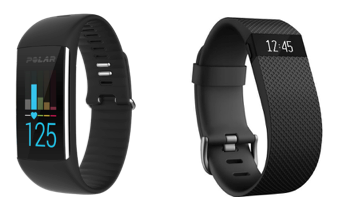
\includegraphics[height=1.9in,width=3in]{wearables} 
		\caption{Example Products used to measure heart rate.\label{fig:wearables}} 
	\end{center} 
\end{figure}

Many of the heart rate monitors use one or more light-emitting diode (LED) optical sensors. 
These heart rate monitors work based on a principle known as Photoplethysmography (PPG) \cite{alian2014photoplethysmography}. Some of these sensors are worn on the arm (e.g., smart 
watches or bands), while others are built into headsets. Although these devices are prolific, 
they often provide inaccurate results \cite{parak2014evaluation}. Advanced signal processing 
and data fusion with other sensors may be used int he future to improve the 
accuracy of this technology.\\

In this report a model and simulation of the heart rate and corresponding Electrocardiography (ECG) \cite{pai2014Electrocardiogram} signals for different physical activities (walking, running, etc) is
described. Additionally, variables such as age, gender, etc. are also included in the model. Further, 
algorithms for extracting heart rate from an ECG signal are developed and included in the simulation.
Such a simulation will provide a test bed for researchers investigating the improvements to wearable
heart rate monitors as described above. The values obtained from the simulation are validated using 
experimental data collected from sensors attached to a human test subject.  

\subsection{Electrocardiogram (ECG) Overview}
An electrocardiogram (ECG) signal is measured as the potential difference (voltage) between  
electrodes placed on the chest. The voltage is caused by ionic current flow which causes the cardiac 
fibers to contract and subsequently relax (the heart pumping action) \cite{mcsharry2003dynamical}. 
Data obtained from ECG signals provides invaluable information for diagnosing cardiac disorders 
which can be extracted using various signal processing techniques \cite{smith2002heart}. ECG 
machines are typically employed in hospitals and medical centers. An example normal cycle ECG 
(representing the successive atrial depolarization/repolarization and ventricular 
depolarization/repolarization \cite{mcsharry2003dynamical}) is displayed in Fig. \ref{fig:ecg}.\\

\begin{figure}[H]
	\begin{center} 
		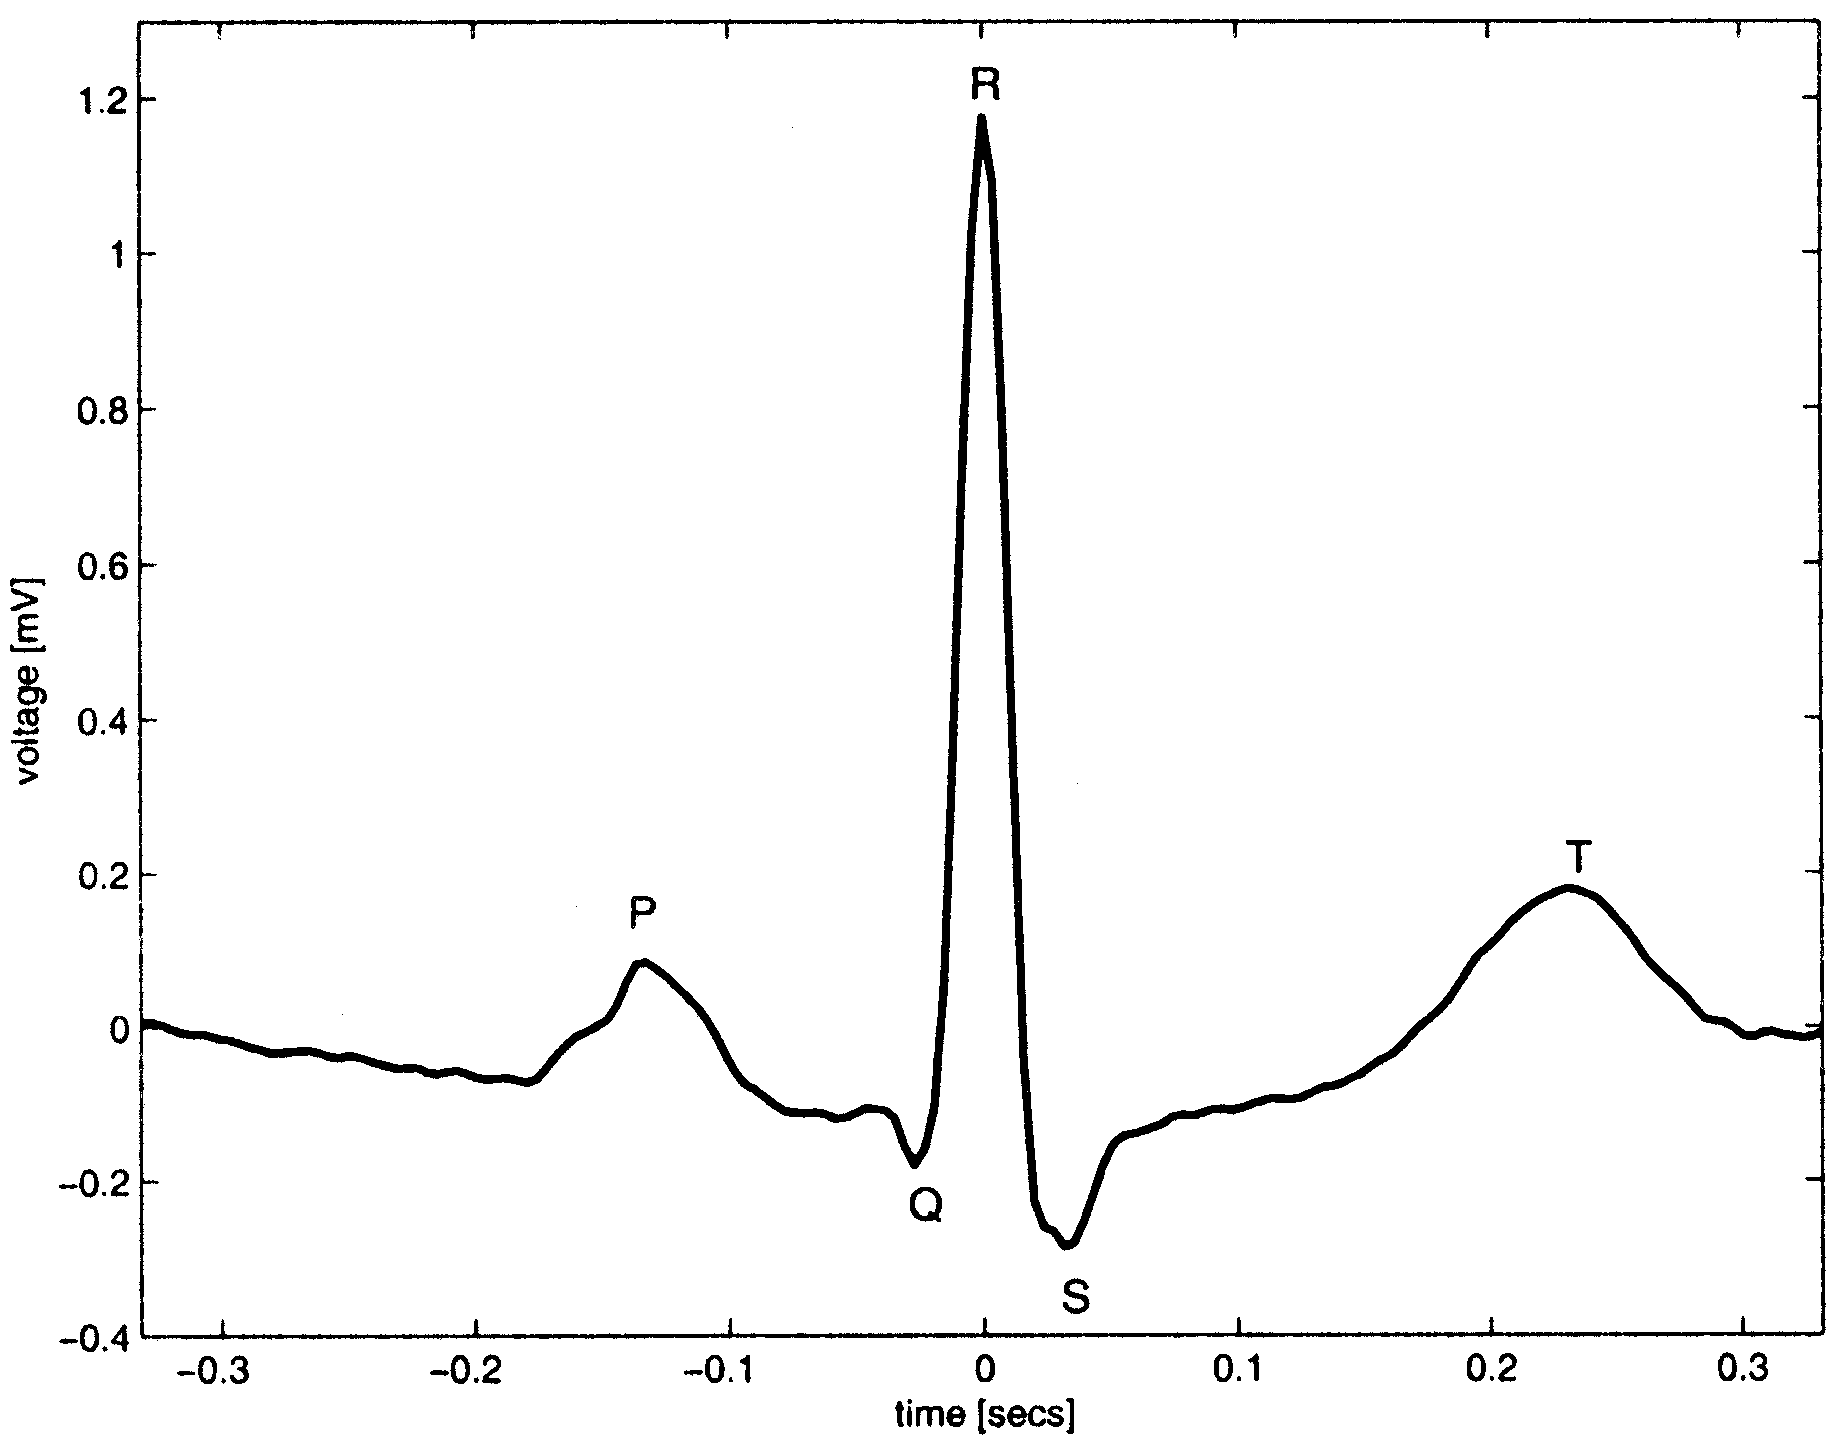
\includegraphics[height=3.14in,width=4in]{mcsharry2003dynamical_ecg} 
		\caption{Example ECG Signal (one cycle) \cite{mcsharry2003dynamical}\label{fig:ecg}} 
	\end{center} 
\end{figure}

However, ECG signals recorded from electrocardiograph require a longtime to setup and can't be used 
for real-time measurements. They can also be corrupted by noise attributed to several factors 
\cite{ackora2013artificial}. Given the importance of having an accurate heart rate measurement, 
since many of the medical decisions will based on that value, there is a need to develop enhanced 
methods and models to accurately estimate HR.\\

In order to effectively detect cardiac abnormalities and monitor rehabilitation exercise, an 
effective way is to set up models for normal heart rate responses. Then, abnormal response detection
can be treated as a fault detection problem. The most commonly used method of fault detection is 
model based residual analysis \cite{blanke2003staroswiecki}. Based on the setup models, abnormal 
responses can be detected by calculating the residual of heart rate response, which can be acquired 
by comparing the signals, measured by using sensor and estimated by using the model. \\

Several researchers have been working on this problem utilizing both experiments and modeling. 
A survey of the relevant literature is presented in the following section. \\

%%%%%%%%%%%%%%%%%%%%%%%%%%%%%%%%%%%%%%%%%%%%%%%%%%%%%%%%%%%%%%%%%%%%%%%%%%%%%%%%%%%%%%%%%%%%%%%%%%%%
\section{Summary of Literature Review}
For this project an extensive review of the literature on synthetic ECG generation as well as heart 
simulation models was conducted. A summary of this review is provided below.\\

% Heart Function
In Ch. 3 of \emph{Physical activity and health: a report of the Surgeon General} 
\cite{united1996physical}, the physiological response of the human body to exercise is discussed.
In particular the response of the cardiac system is detailed which provided helpful insight for 
the development of this simulation.\\

% Simulating HR
A model for simulation HR based on activity level is given in \emph{Simulation of living behavior: 
a cardiovascular model for predicting blood pressure and heart rate} \cite{hotehama2003simulation}.
The authors use the required oxygen levels for various activities to calculate the heart rate 
required to deliver that amount of oxygen to the body. Various factors impact this calculation 
such as the Stroke Volume (SO) of the heart and the amount of oxygen content in the blood. This 
paper, along with its references, provides the basis for the HR simulations developed in this
project.\\

% Processing HR
Su, et al \cite{su2010dynamic} investigated human heart rate response dynamics to moderate 
exercises. A healthy male subject was considered to walk on a motorized treadmill under a predefined
exercise protocol. ECG, body movements, and oxygen saturation were monitored and recorded by using 
non-invasive portable sensors.  They reduced the variation heart rate measurement caused by the 
influence of various internal or external factors by considering a step response protocol that has 
been repeated three times. The experimental results show that both steady state gain and time 
constant of heart rate response are not invariant when walking speed is faster than 3 miles/hour, 
and time constant of offset exercise is noticeably longer than that of onset exercise.\\

% Processing HR
Su, et al proposed a novel integrated approach for the identification and control of Hammerstein 
systems to achieve desired heart rate profile tracking performance for an automated treadmill 
system. The proposed algorithm achieved much better heart rate tracking performance 
\cite{su2007identification}.\\

% Processing HR
Hunt, et al considered the identification of the heart dynamics during moderate-to-vigorous 
treadmill exercise and explored parameter dependencies with respect to time, intensity level and 
step-change direction \cite{su2007identification}. There are several systems for feedback control of
HR that can be conveniently implemented on cycle ergometers \cite{paradiso2013experimental} or 
treadmills; the aim is to automatically set the cycling load or treadmill speed to achieve a 
prescribed target HR intensity.\\

% Synthetic ECG signal
The authors of \emph{A Dynamical Model for Generating Synthetic Electrocardiogram Signals} 
\cite{mcsharry2003dynamical} develop a model for generating synthetic ECG signals that can be 
adjusted to represent different scenarios (low signal to noise, various sample rates, etc.).
Such a model can may be employed to assess biomedical signal processing techniques which are used 
to compute clinical statistics from the ECG. The model presented represents the ECG signal as a 3-D 
periodic signal traveling around in a circle. The amplitude (z direction) of the signal changes to 
represent the events during the cycle. The locations of these events are determined by angles 
(locations in the circle). Variations in the length of the RR interval can be achieved by varying 
the angular velocity at which the signal travels around the circle. Complex features of the HR 
(e.g. HRV) can be accounted for by this model. The operator can select specific characteristics 
about the HR such as mean, SD, and spectral properties like LF/HF ratio (corresponds to HRV).\\

% Synthetic ECG signal
In the paper \emph{Simulating Healthy Human Heart Rate: A Markovian Model} \cite{yang2002simulating}
the authors create a synthesized ECG signal utilizing a probability table created from real  data 
sets. A Markovian model was developed to determine state transitions (decreasing and increasing 
heart rate) based on the constructed probability tables and the previous states. This is not a 
simulation of heart activity based on external inputs but rather a method for generating synthetic 
ECG signals for analysis. This is similar to the desire of this project; however, the control of the
ECG signal is entirely dependent on the table of analyzed data and not general.\\

% Synthetic ECG signal
In \emph{An Artificial ECG Signal Generating Function in MATLAB} \cite{ackora2013artificial}
The authors develop a method to mathematically generate ECG signals given HR and peak voltage as 
inputs. This allows the generation of many different ECG signals for analysis. The function is 
developed in MATLAB\textsuperscript{TM} and outputs a 10 second ECG signal based on inputs of average 
HR and maximum signal level. The functional concept was implemented in this project. \\

% Synthetic ECG signal
The characteristics of Heart Rate Variability (HRV) are used in \emph{Heart Rate Variability 
	Characteristics Required for Simulation of Interval Sequences} \cite{smith2002heart} to classify
real and synthesized R-to-R interval
\footnote{The inverse of the R-to-R interval (RR Interval) is Heart Rate 
	\cite{mcsharry2003dynamical}.}
data (essentially ECG signals). The data was analyzed in both
the time domain and frequency domain in order to extract HRV characteristics.\\

% Synthetic ECG signal
McSharry et al. introduced an appropriate dynamical model for Electrocardiogram (ECG) signal 
based on its morphology which is capable of generating synthetic ECG signals
\cite{mcsharry2003dynamical}.\\

% Synthetic ECG signal
Boulakia  et al. dealt with the numerical simulation of electrocardiograms (ECG). The goal was to 
devise a mathematical model, based on partial differential equations, which is able to provide 
realistic 12-lead ECGs. The numerical ECGs obtained with this approach showed correct amplitudes, 
shapes and polarities, in all the 12 standard leads \cite{boulakia2010mathematical}.\\

% Synthetic PCG signals
Almasi, et al. introduced a dynamical model for Phonocardiogram (PCG) signal which is capable of 
generating realistic synthetic PCG signals. The model was based on PCG morphology and consists of 
three ordinary differential equations and can represent various morphologies of normal PCG signals. 
This model can be employed to assess biomedical signal processing techniques
\cite{almasi2011dynamical}.\\

% Processing ECG
Sameni, et al. reviewed a range of promising recording and signal processing techniques for fetal 
ECG analysis that have been developed over the last forty years, and discuss both their shortcomings 
and advantages \cite{sameni2010review}.

%%%%%%%%%%%%%%%%%%%%%%%%%%%%%%%%%%%%%%%%%%%%%%%%%%%%%%%%%%%%%%%%%%%%%%%%%%%%%%%%%%%%%%%%%%%%%%%%%%%%
\section{Conceptual Model Development} \label{sec:model}
The conceptual model is a representation of the System Under Investigation (SUI) using some type of 
formalism. It is an abstraction of a real world system and it is essential to the successful 
development of a simulation program representing the SUI \cite{robinson2013conceptual}. The role of 
the conceptual model is shown below in Figure \ref{fig:01}. \\
	
\begin{figure}[H]
	\begin{center} 
		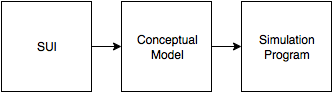
\includegraphics[height=1in,width=3.6in]{sui_mod_sim} 
		\caption{The role of the conceptual model\label{fig:01}} 
	\end{center} 
\end{figure}

\subsection{Objective} \label{sec:model_obj}
For this project, the objective is to model the heart rate for different physical activities 
(walking, running, etc) considering values such as age, gender, etc. As well as generating the
corresponding ECG signals and processing the generated ECG signals.

\subsection{Input} \label{sec:model_in}
Model inputs include characteristics of the human being modeled (mass, resting HR, etc.) as well
as data detailing the levels of physical activity (intensity, duration, etc.). The required 
inputs for describing parameters of the human who's heart rate will be calculated are shown in
Table \ref{tbl:human}. 

\begin{table}[h]
	\centering
	\caption{Model Inputs: Human}
	\label{tbl:human}
	\begin{tabular}{|l|l|}
		\hline
		\textbf{Inputs} & \textbf{Units} \\ \hline
		Mass            & kg             \\ \hline
		Resting HR      & beats/min      \\ \hline
		$VO_{2max}$     & MET            \\ \hline
	\end{tabular}
\end{table}

Average coefficients for blood oxygen saturation ($VO_{2max}$) can be calculated based on 
physical characteristics (age, gender, etc.) \cite{balady1995exercise}. The blood oxygen 
saturation coefficient represents the maximal oxygen of the human. The average $VO_{2max}$ 
values for age and gender categories are shown below in Table \ref{tbl:vo2max}.

\begin{table}[h]
	\centering
	\caption{Average coefficients for blood oxygen saturation at different ages
		\cite{balady1995exercise}}
	\label{tbl:vo2max}
	\begin{tabular}{|l|l|l|}
		\hline
		\textbf{Age (yrs)} & \textbf{Men} & \textbf{Women} \\ \hline
		20-29              & 12           & 10             \\ \hline
		30-39              & 12           & 10             \\ \hline
		40-49              & 11           & 9              \\ \hline
		50-59              & 10           & 8              \\ \hline
		60-69              & 9            & 8              \\ \hline
		70-79              & 8            & 8              \\ \hline
	\end{tabular}
\end{table}

The required inputs (parameters) for describing activities are shown in 
Table \ref{tbl:activities}.

\begin{table}[h]
	\centering
	\caption{Model Inputs: Activities}
	\label{tbl:activities}
	\begin{tabular}{|l|l|}
		\hline
		\textbf{Inputs}    & \textbf{Units} \\ \hline
		Start Time         & min            \\ \hline
		Duration           & min            \\ \hline
		Intensity          & MET            \\ \hline
		Type (Description) & Text           \\ \hline
	\end{tabular}
\end{table}

Physical activity will be described in units of METs \footnote{One MET is the resting level of 
metabolic activity for the average person and is equivalent to 3.5 ml of oxygen per kilogram of 
body mass per minute (3.5 ml/kg/min) \cite{hotehama2003simulation}.}. The intensity (in units
of MET) for various activities can be found in \cite{ainsworth2000compendium}. Some example 
values are displayed below in Table \ref{tbl:mets}.

\begin{table}[H]
	\centering
	\caption{Intensities for various activities in METs \cite{ainsworth2000compendium}}
	\label{tbl:mets}
	\begin{tabular}{|l|l|}
		\hline
		\textbf{Activity Description} & \textbf{Intensity (METs)} \\ \hline
		Sleeping                      & 0.92                      \\ \hline
		Grocery Shopping              & 2.1                       \\ \hline
		Walking                       & 3.8                       \\ \hline
		Dancing                       & 4.5                       \\ \hline
		Running                       & 7.5                       \\ \hline
	\end{tabular}
\end{table}

\subsection{Output} \label{sec:model_out}
The model output is a synthesized ECG signal trace (see example in Fig. \ref{fig:ecg}) that 
can be processed to get information. Different ECG signal processing algorithms can be tested
on the data output from this simulation.

\subsection{Content} \label{sec:model_cont}
The content of the conceptual model is divided into two parts: the HR simulation, and the ECG
signal synthesis. The ECG synthesis relies on input from the HR simulation. The HR conceptual
model turned out to be one of the most difficult aspects of this project due to lack of 
similar work documented in the literature. The paper by Hotehama et. al.
\cite{hotehama2003simulation} was the only paper that described a model similar to what we
desired for this project.

\subsubsection{Heart Rate Calculation}\label{sec:model_cont_hr}
If the amount of oxygen required by a physical activity is known, the heart rate required to 
deliver that oxygen to the body can be calculated \cite{hotehama2003simulation}. The amount of 
oxygen supplied to the body is a product of the cardiac output (CO) and the oxygen content in the
blood which is known as the arteriovenous oxygen content difference ($C_{av}$)
\cite{hotehama2003simulation}. The CO (ml/min) is a product of HR and stroke volume (SV)
\cite{stringer1997cardiac}.

\begin{equation}\label{eq:co}
CO = SV * HR
\end{equation}

As described in section \ref{sec:model_in}, average coefficients for blood oxygen saturation 
($VO_{2max}$) can be calculated based on physical characteristics (age, gender, etc.) 
\cite{balady1995exercise}. An equation for the arteriovenous oxygen content difference ($C_{av}$ in 
units of ml/100ml) based the amount of exercise intensity (in units of METs) as a percentage of 
$VO_{2max}$ was developed by Stringer et. al. \cite{stringer1997cardiac} and is shown in Eq. 
\ref{eq:cav}.

\begin{equation}\label{eq:cav}
C_{av} = 5.72 + (0.1047 * \%VO_{2max}) 
\end{equation}

The volume of oxygen consumed by a human during physical activity per minute is calculated by the
mass (M) of the individual (kg) multiplied by the intensity of the activity (I) in METs. This leads
to the following equation.

 \begin{equation}\label{eq:oxy}
 M*3.5*I=SV*HR*C_{av}/100
 \end{equation} 

From Eq. \ref{eq:oxy} it is evident that given the inputs described in section \ref{sec:model_in}
and the SV, the HR can be calculated. The SV changes as the heart is put under more load (increased
blood pressure) and must therefore be modeled as changing with exercise intensity 
\cite{hotehama2003simulation}. During exercise, the SV will increase until approximately at 40 to 
60\% of $VO_{2max}$ is reached \cite{united1996physical}. After analyzing experimental data from 
\cite{united1996physical}, the SV is modeled as a linear function that plateaus at a 65\% 
increase in the initial SV when 60\% of $VO_{2max}$ is reached. The initial SV (at rest) 
is calculated by Eq. \ref{eq:sv} (here HR is equivalent to the individual's resting HR and I is
equal to 1 MET).

\begin{equation}\label{eq:sv}
SV = HR*C_{av}/100/M/3.5
\end{equation}

With an equation developed for SV the HR can now be calculated for various activities given the 
inputs discussed in section \ref{sec:model_in}.

\subsubsection{ECG Signal Generation}\label{sec:model_cont_ecg}
The methodology for the ECG signal generation follows the method published in 
\cite{mcsharry2003dynamical} and will be described briefly in this section. \\

The model is based on a dynamical system with three coupled ordinary differential equations 
which is capable of generating realistic synthetic electrocardiogram (ECG) signals. The model 
also depends on the morphology of the PQRST cycle as shown in Fig. \ref{fig:ecg} and the power 
spectrum of the RR tachogram for both respiratory sinus arrhythmia at the high frequencies (HFs)
and Mayer waves at the low frequencies (LFs) together with the LF/HF ratio.\\

The coupled system is shown in the equations below \cite{mcsharry2003dynamical}. The value of 
z will provide the ECG signal as a function of sampling frequency and time.

\begin{equation}\label{eq:ecg1}
\begin{split}
\alpha = \sqrt{x^2 + y^2} \\
\Delta\theta_i = (\theta - \theta_i)mod 2\pi \\
\theta = atan2(x,y)
\end{split}
\end{equation}

\begin{equation}\label{eq:ecg2}
\dot{x}=\alpha x + \omega y
\end{equation}

\begin{equation}\label{eq:ecg3}
\dot{y}=\alpha y + \omega x 
\end{equation}

\begin{equation}\label{eq:ecg4}
\dot{z} = -\sum a_i \Delta\theta_i exp\left(\frac{\Delta\theta_i^2}{2b_i^2}\right) - (z - z_0)
\end{equation}

Note that z0 is given as

\begin{equation}\label{eq:ecg5}
z_0(t) = A sin(2\pi f_2t)
\end{equation}

where A is given as 0.15 mV and $f_2$ and $f_1$ are given as 0.1, 0.25 respectively. The 
RR-interval time series $T(t)$ with power spectrum $S(f)$ is generated by taking the inverse 
Fourier transform of a sequence of complex numbers with amplitudes $\sqrt{S(f)}$ which is 
given as

\begin{equation}\label{eq:ecg6}
S(f) = \frac{\sigma^2_1}{\sqrt{2\pi c^2_1}}exp\left(\frac{(f-f_1)^2}{2c_1}\right) +
       \frac{\sigma^2_2}{\sqrt{2\pi c^2_2}}exp\left(\frac{(f-f_2)^2}{2c_2}\right) 
\end{equation}

where c1 and c2 is given as 0.01. The time-dependent angular velocity of motion around the limit
 cycle is given by

\begin{equation}\label{eq:ecg7}
\omega(t) = \frac{2\pi}{T(t)}
\end{equation}

This model for the ECG signal generation is discussed further (including pseudo code) in 
section \ref{sec:simdev_ecg}. 

\subsection{Assumptions and Simplifications} \label{sec:modle_ass}
Several approximations for have to be made for the HR simulation. The authors in
\cite{hotehama2003simulation} estimated SV by developing a trend line using measured data. In 
this model experimental data from \cite{united1996physical} is used to develop a linear 
approximation. In reality there are many factors that can effect the exact SV curve (e.g.,
thermal stress can effect SV \cite{wilson2011effect}).\\

Heart rate change is not instantaneous and is modeled here as linear transition taking two 
minutes \cite{hotehama2003simulation}\cite{koga1996pulmonary}\cite{carter2000effect}. Further,
$VO_2$ drift at high activity levels (intensity greater than 6 METs) 
\cite{hotehama2003simulation}\cite{carter2000effect} is not taken into consideration.

%%%%%%%%%%%%%%%%%%%%%%%%%%%%%%%%%%%%%%%%%%%%%%%%%%%%%%%%%%%%%%%%%%%%%%%%%%%%%%%%%%%%%%%%%%%%%%%%
\section{Simulation Development} \label{sec:simdev}
The simulation developed for this project is divided into three sections: the heart rate
simulation, the ECG calculations, and the ECG post processing. Each of these three simulations
are discussed below.

\begin{figure}[H]
	\begin{center} 
		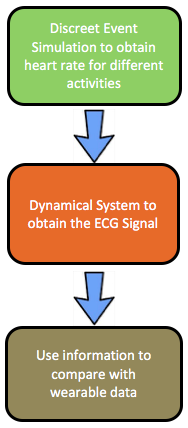
\includegraphics[height=3in,width=1.32in]{simulation_outline} 
		\caption{Process flow to obtain the synthetic ECG signal. \label{fig:sim_outline}} 
	\end{center} 
\end{figure}

\subsection{Heart Rate Simulation Development}\label{sec:simdev_hr}
The HR simulation is based on the concept of a Discrete Event Simulation (DES). Each activity
start and activity end represents a discrete event. As the input file (see sections 
\ref{sec:model_in} and appendix \ref{sec:A:map}) is processed, activity objects are created and 
put into a priority queue that is sorted based on the activity's start time (smallest start time
first). This queue is called the Future Event List (FEL). A priority queue based on a heap data 
structure \footnote{https://docs.python.org/2/library/queue.html} is used to implement the FEL. \\

As events are popped out of the queue they are handled by a ``start activity'' event handler. 
Inside the event handler, the parameters of the activity are used to calculate the HR required
for the activity using the equations developed in section \ref{sec:model_cont}. When each 
starting event is processed, an ``end activity'' event is scheduled in the FEL. When the ``end 
event'' is processed the HR is returned to the resting state.\\

Once the DES has completed the generated list of HR changes are reprocessed and transitions
are added. The HR transitions are modeled as linear transitions that take two minutes. This
transition is modeled as discrete steps each 10 seconds long. 

\subsection{Electrocardiogram Simulation Development}\label{sec:simdev_ecg}
The ECG simulation solves a system of ordinary differential equations (described in section
\ref{sec:model_cont_ecg}). An ODE solver
\footnote{http://docs.scipy.org/doc/scipy/reference/generated/scipy.integrate.odeint.html}
is used to solve for the ECG signal. A RNG is used to create simulated measurement noise
which is added to the signal. The RNG used is described in appendix \ref{sec:A:rng}. \\

The average heart rate calculated from the DES described in the previous section is given 
as an input to the ECG simulation. Pseudo code for the ECG simulation is provided below.\\

\lstset{language=Matlab}
\begin{lstlisting}[frame=single, caption={ECG Pseudo Code}, label=ecg_code1]
% Inputs:
Fs = 100                    % Sampling frequency (samples/sec)
sfecg = sfinit = Fs         % ECG sampling frequency [Hertz]
M = 10                      % Approximate number of heart beats
Anoise = 0                  % Additive uniformly distributed noise [0 mV]
hrmean = 60                 % Mean heart rate [60 beats per minute]
hrstd = 1                   % Standard deviation of HR [1 beat/minute]
lfhfratio = 0.5             % low-frequency/high-frequency (LF/HF) ratio [0.5]
ti = [-60 -15 0 15 90]      % P  Q  R  S  T   ti = angles of extreme degrees
ti = ti*pi/180              % convert to radians
ai = [1.2 -5 30 -7.5 0.75]  % z-position of extreme 
bi = [0.25 0.1 0.1 0.1 0.4] % Gaussian width of peaks 
flo = 0.1                   % frequency parameters (Mayer waves)
fhi = 0.25                  % frequency parameters (respiratory rate)
flostd = 0.01               % f10 standard deviation  
fhistd = 0.01               % fhi standard deviation  
n = M                       % Constant used in the RR interval calculation 

% Output (ECG): 
% Compute the RR-interval which is the time between successive 
% R-peaks, the inverse of this time interval gives the 
% instantaneous heart rate.
hrfact = sqrt(hrmean/60.0)
hrfact2 = sqrt(hrfact)
bi = hrfact*bi
ti = [hrfact2, hrfact, 1., hrfact, hrfact2]*ti
q = round(sfint/sfecg)

sfrr = 1.0  			% Sampling frequency
w1 = 2*pi*flo
w2 = 2*pi*fhi
c1 = 2*pi*flostd
c2 = 2*pi*fhistd
sig2 = 1.
sig1 = lfhfratio
rrmean = 60/hrmean
rrstd = 60*hrstd/(hrmean*hrmean)

df = sfrr/n
w = arange(n)*2*pi*df
dw1 = w - w1
dw2 = w - w2

% Power spectrum of the RR-intervals
Hw1 = sig1*exp(-0.5*(dw1/c1)^2)/sqrt(2*pi*c1^2)
Hw2 = sig2*exp(-0.5*(dw2/c2)^2)/sqrt(2*pi*c2^2)
Hw = Hw1 + Hw2

% An RR-interval time series with power spectrum is generated by taking 
% the inverse Fourier transform of a sequence of complex numbers with 
% amplitude sqrt of Hw
Sw = (sfrr/2)*sqrt(Hw)
ph0 = 2*pi*rand(n/2-1,1)
ph = [0; ph0; 0; -flipud(ph0)]
SwC = Sw*exp(1j*ph)
x = (1/n)*real(ifft(SwC))  
xstd = std(x)
ratio = rrstd/xstd
RR = rrmean + x*ratio
RR = interp(linspace(0, len(RR) - 1, len(RR)*sfint), range(len(RR)), RR)
dt = 1/sfint

% Solve the ODE system  shown below 
t_span = arange(start=dt, stop=len(x), step=dt)  
x0 = [1, 0, 0.04]
sol = odeint(Function, x0, t_span, args=(0, RR, sfint, ti, ai, bi))
\end{lstlisting}

\subsection{ECG Processing Algorithm}
An ECG signal must be post processed in order to determine the useful information. The main piece
of information is the average HR. The algorithm used to process the experimental data utilizes a
peak search algorithm to count the number of peaks. This count is then divided by the amount of 
elapsed time to get HR in beats per minute. This particular script was implemented in MATLAB to
process the experimental data. A similar algorithm could be used to process the synthetic ECG 
signals created by this simulation.

%%%%%%%%%%%%%%%%%%%%%%%%%%%%%%%%%%%%%%%%%%%%%%%%%%%%%%%%%%%%%%%%%%%%%%%%%%%%%%%%%%%%%%%%%%%%%%%%%%%%
\section{Description of Simulation Software} \label{sec:software}
The simulation software was developed in Python. The main function is displayed below with detailed 
explanation of its use following.

\newpage
\lstset{language=Python}
\begin{lstlisting}[frame=single, caption={Simulation Main Function}]
def main():
	
  # -------- User Inputs and Settings -------------------------------------- #
	
  # The content of the input file describes characteristics of the human and
  # their different activities.
  input_file_path = "input_short.txt"

  # Output file paths
  ecg_file_path = "output_ecg.txt"
  hr_file_path = "output_hr.txt"

  # If the verbose flag is set details are printed to the console.
  verbose = True

  # If the visual flag is set simulation outputs are plotted.
  # Note: Each plot window must be closed to alow the simulation to continue.
  visual = True

  # ------------------------------------------------------------------------ #

  # Read input file and create the human object and queue of activities.
  human, fel = read_input_file(input_file_path, verbose=verbose)

  # Create the HR simulation object
  hr_sim = HeartSimulation(human, fel, verbose=verbose, visual=visual)

  # Run the simulation
  hr_sim.run_simulation(hr_file_path)

  # Generate the ECG signals (store in file for separate processing)
  ecg_sim = ECGSimulation(hr_sim.avg_hr, visual=visual)
  ecg_sim.run_simulation(file_path=ecg_file_path)
  
\end{lstlisting}
\vspace{2mm}

The main function is broken into two parts: the user input settings and the simulation. The user
inputs are file paths for the input and output files. The input file is described in appendix 
\ref{sec:A:map}. The output files log the generated data. The ECG data file can get quite large
due to the high sample rate required for the displaying the fine detail of the ECG signal. The
``verbose'' flag is used to turn text output (printed to the terminal) on and off. When the 
``visual'' flag is set the simulation will generate plots of the data as it is generated. With 
both flags set to false only the output files will be generated.\\

The simulation is handled by two main objects: the ``HeartSimulation'' object and the 
``ECGSimulation'' object. These objects contain the simulation code described in previous sections.

%%%%%%%%%%%%%%%%%%%%%%%%%%%%%%%%%%%%%%%%%%%%%%%%%%%%%%%%%%%%%%%%%%%%%%%%%%%%%%%%%%%%%%%%%%%%%%%%%%%%
\section{Simulation Results}
This section discusses some of the simulation results. The results are compared with measured and
other metrics to determine validity.

\subsection{HR Simulation Results}
The output from the HR DES is shown in the following two plots. The output was generated by giving
the simulation the input file shown in appendix \ref{sec:A:map}.

\begin{figure}[H]
	\begin{center} 
		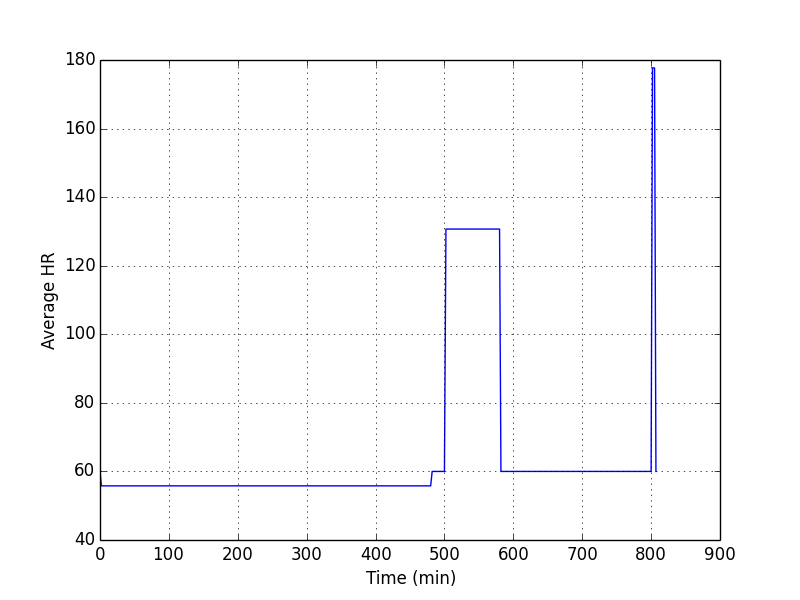
\includegraphics[height=3in,width=4in]{avg_hr} 
		\caption{Simulated Average HR. \label{fig:hr}} 
	\end{center} 
\end{figure}

\begin{figure}[H]
	\begin{center} 
		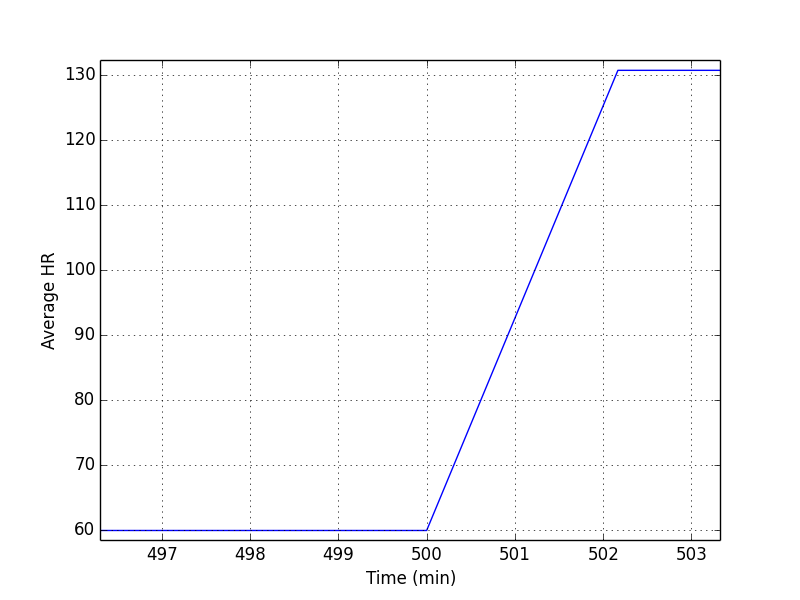
\includegraphics[height=3in,width=4in]{avg_hr_zoomed} 
		\caption{Simulated Average HR (zoomed to show transition). \label{fig:hr_zoom}} 
	\end{center} 
\end{figure}

\subsubsection{HR Simulation Validation}
In order to validate the HR simulation, the calculated values were compared against average values
in the literature (or otherwise public knowledge). Several of the calculated values used for 
validation are summarized in Table .

\begin{table}[H]
	\centering
	\caption{HR Simulation Validation}
	\label{tbl:hr_valid}
	\begin{tabular}{lll}
		\hline
		\textbf{Value}        & \textbf{Simulation} & \textbf{Liturature} \\ \hline
		Max HR                & 177 beats/min       & 190 beats/min       \\
		Target HR             & 130 beats/min       & 133 beats/min       \\
		Resting Stroke Volume & 70 ml               & 70 ml              \\ \hline
	\end{tabular}
\end{table}

The maximum HR simulated was calculated during maximum intensity for the simulated human (in this 
case 12 METs). An estimate for a human's maximum HR is given by subtracting the human's age
from 220 \cite{mayo2014exercise} (in this case 30 years). The target HR for exercising is calculated 
as 70\% of the maximum HR \cite{mayo2014exercise}. The simulated value was calculated during an
exercise intensity of four METs. It is important to note that the simulation results will vary 
depending on the characteristics of the simulated human (e.g., resting HR, mass, etc.). These
values are intended to show the simulation produces realistic values for average HR.
The normal stroke volume used for comparison was obtained from \cite{klabunde1015regulation}.

%%%%%%%%%%%%%%%%%%%%%%%%%%%%%%%%%%%%%%%%%%%%%%%%%%%%%%%%%%%%%%%%%%%%%%%%%%%%%%%%%%%%%%%%%%%%%%%%%%%%
\subsection{ECG Simulation Results}
Some of the input into the model is shown below in Fig. \ref{fig:ecg_params}. The ECG signal for an
average heart rate of approximately 60 beat per minute as a function of time is shown in Fig.  
\ref{fig:sim_ecg}. Note that this model also includes noise to represent actual data more 
realistically. 

\begin{figure}[H]
	\begin{center} 
		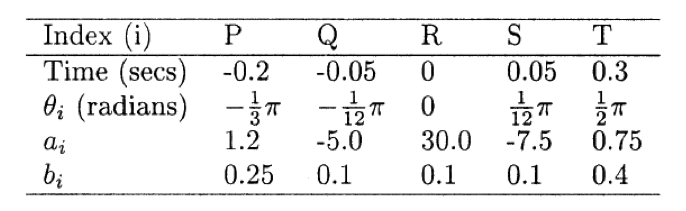
\includegraphics[height=.91in,width=3in]{ecg_params} 
		\caption{Parameters of the ECG Model \cite{mcsharry2003dynamical}. \label{fig:ecg_params}} 
	\end{center} 
\end{figure}

\begin{figure}[H]
	\begin{center} 
		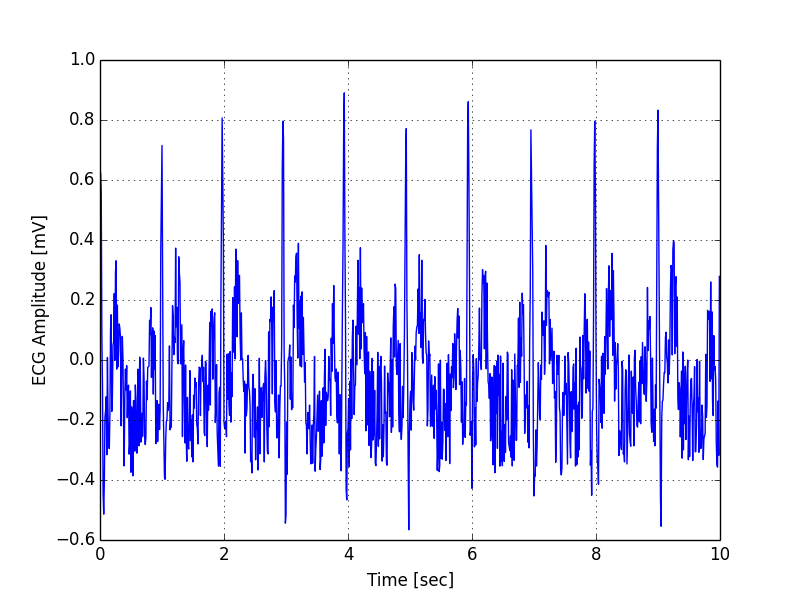
\includegraphics[height=3in,width=4in]{sim_ecg} 
		\caption{ECG generated by dynamical model. \label{fig:sim_ecg}} 
	\end{center} 
\end{figure}

\subsubsection{ECG Simulation Validation}
Experimental HR data was analyzed in order to validate the simulation output. The experimental
data is presented in appendix \ref{sec:A:exp}. By comparing the behavior of both experiments 
and simulation we notice that we obtain a very similar representation (note that the values of 
the simulation is scaled so the reader should only refer to the general behavior of the signal).
  
%%%%%%%%%%%%%%%%%%%%%%%%%%%%%%%%%%%%%%%%%%%%%%%%%%%%%%%%%%%%%%%%%%%%%%%%%%%%%%%%%%%%%%%%%%%%%%%%
\section{Summary}
In this report a model was developed for simulating the HR and subsequent ECG signal given 
specific attributes of a human and a list of different physical activities (e.g., sleeping, 
running, etc.). The HR simulation is based on the concept of a discrete event simulation (where
each change in activity is a discrete event) and is used to provide input to the ECG simulation.
The ECG simulation is a dynamical system described by couple differential equations. An ODE
solver was used to perform the calculation. Experimental data was taken and compared with the 
simulated output visually for validation. A complete example simulation is presented in appendix 
\ref{sec:A:sim}. \\

This output of this simulation can be used to aid active health monitoring within wearable
technologies. Additionally, the simulated signals can be used to test ECG processing algorithms
without the need to acquire experimental data. 

%%%%%%%%%%%%%%%%%%%%%%%%%%%%%%%%%%%%%%%%%%%%%%%%%%%%%%%%%%%%%%%%%%%%%%%%%%%%%%%%%%%%%%%%%%%%%%%%%%%%
%%% Appendices
\newpage
\begin{appendices}

%%%%%%%%%%%%%%%%%%%%%%%%%%%%%%%%%%%%%%%%%%%%%%%%%%%%%%%%%%%%%%%%%%%%%%%%%%%%%%%%%%%%%%%%%%%%%%%%%%%%
\section{Experimental Data Collection}\label{sec:A:exp}
This section descries the experimental data obtained by considering several optical sensors attached 
to the body. The mean value of the heart rate will be considered by averaging all the results from 
the 3 sensors. The experimental setup is shown in Fig. \ref{fig:exp}. An Arduino and an XD-58C Pulse 
sensor Heart-rate sensor module for Arduino was used to capture the HR. A laptop in this case was
used to store the data and perform analysis. \\

\begin{figure}[H]
	\begin{center} 
		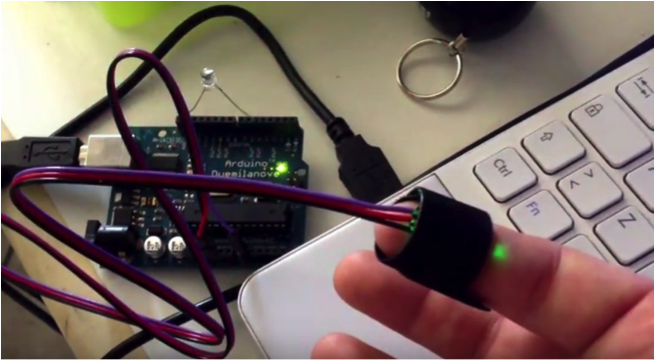
\includegraphics[height=2in,width=3.6in]{hr_experiment} 
		\caption{Experimental setup to obtain heart rate.\label{fig:exp}} 
	\end{center} 
\end{figure}

The raw data obtained from the three sensors as a function of time is displayed in Fig. 
\ref{fig:measdat}. The computed heart rate (HR) is shown in Fig. \ref{fig:measbpm}. Note that the
HR is simply the number of peaks observed in the raw data divided by time to obtain beat per minute.
Considering the entire dataset as a whole the average BPM is 77. This data set is utilized to validate
the simulations presented in the main body of the report.\\

\begin{figure}[H]
	\begin{center} 
		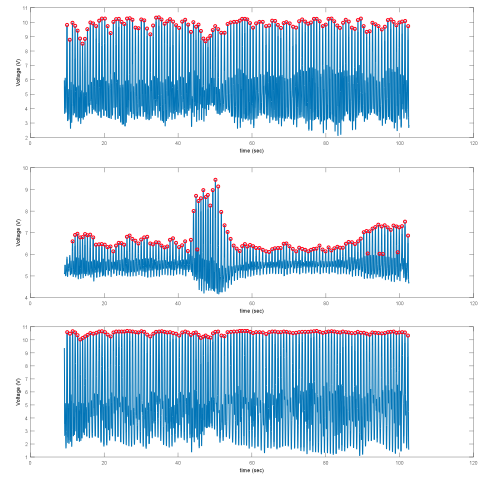
\includegraphics[height=4in,width=4in]{measured_data} 
		\caption{Measured HR signals (voltage [V] vs. time [s]).\label{fig:measdat}} 
	\end{center} 
\end{figure}

\begin{figure}[H]
	\begin{center} 
		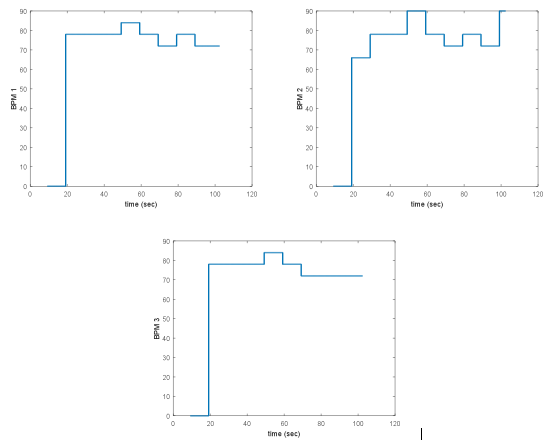
\includegraphics[height=4in,width=5in]{measured_bpm} 
		\caption{Measured HR (BPM vs. time [s]).\label{fig:measbpm}} 
	\end{center} 
\end{figure}

%%%%%%%%%%%%%%%%%%%%%%%%%%%%%%%%%%%%%%%%%%%%%%%%%%%%%%%%%%%%%%%%%%%%%%%%%%%%%%%%%%%%%%%%%%%%%%%%%%%%
\newpage
\section{Random Number Generation}\label{sec:A:rng}
As discussed in the main body of this report, the simulation utilizes randomness 
in several places.
Software algorithms have been created for the purpose of generating pseudo random numbers. 
Since the generation is deterministic (software algorithm) the numbers are not truly 
random; however, the algorithms are designed to generate streams of numbers that are not 
correlateable to the previous samples and hence appear random. The Random Number Generator 
(RNG) implemented is discussed in this appendix.

\subsection{Uniformly Distributed Random Variant}\label{sec:A:rng:uniformrng}
The ``Minimal'' random number generator developed by Park and Miller 
\cite{press1996numerical} was selected to generate a uniform random deviate between 0.0 and 
1.0. The algorithm is presented in \cite{press1996numerical} written in C. It was adapted 
to Python for this project and is presented below.\\

\lstset{language=Python}
\begin{lstlisting}[frame=single, label=some-code, caption=Minimal Random Number Generator]
def min_rand(seed=0):

    # Define constants
    ia = 16807
    im = 2147483647
    am = (1.0/im)
    iq = 127773
    ir = 2836
    mask = 123459876
	
    # Only allow the generator to be seeded once
    if "seed" not in min_rand.__dict__:
        # XORing with MASK allows use of zero and other simple bit patterns
        # for seed.
        min_rand.seed = seed ^ mask

    # Compute idum=(IA*idum) % IM without over-flows by Schrage's method.
    k = min_rand.seed/iq
    min_rand.seed = ia*(min_rand.seed - k*iq) - ir*k
    if min_rand.seed  < 0:
        min_rand.seed += im
    rand_val = am*min_rand.seed  # Convert to a floating result.
    
    return rand_val
\end{lstlisting}
\vspace{2mm}

\newpage
The generator was tested for the desired behavior using the \emph{Chi-Squared} test 
\cite{Navidi2008Stats} as discussed in class (see equation \ref{eqn:chi2}). 

\begin{equation} \label{eqn:chi2}
A_m = \sum_{i=1}^{k} \frac{O_i - E_i}{E_i}
\end{equation} 

\noindent
Where $O_i$ is the number of values in bin $i$ and $E_i$ is the expected value.
The calculated value of $A_m$ is 27 which is much less than $\chi^*$ of 38.885 for 26 degrees of 
freedom (27 bins) and $\alpha = 0.05$. This indicates acceptable performance of the RNG. The set of 
generated random values used for this test is shown graphically in Figure \ref{fig:A:URNG}.\\

\begin{figure}[H]
	\begin{center} 
		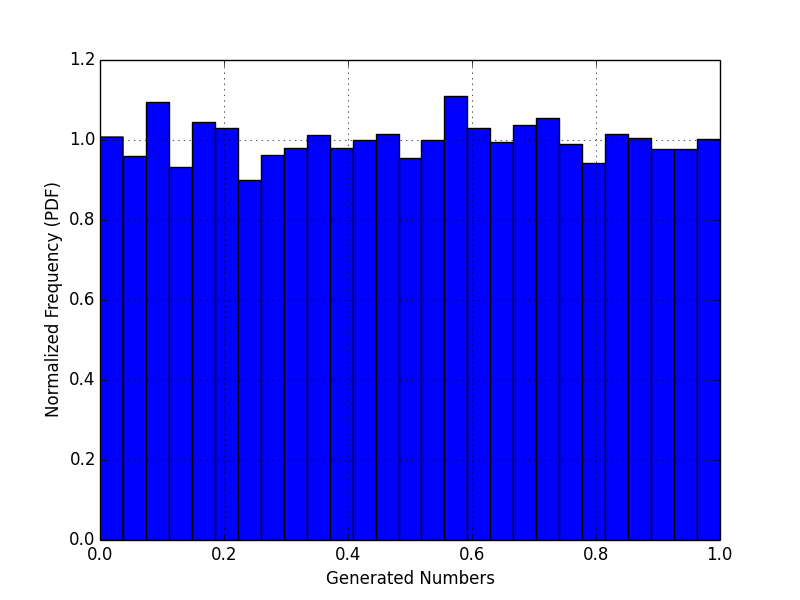
\includegraphics[height=4in,width=5.5in]{uniform_rng} 
		\caption{Histogram of Uniformly Distributed Random Numbers Generated\label{fig:A:URNG}}
	\end{center} 
\end{figure}

%%%%%%%%%%%%%%%%%%%%%%%%%%%%%%%%%%%%%%%%%%%%%%%%%%%%%%%%%%%%%%%%%%%%%%%%%%%%%%%%%%%%%%%%%%%%%%%%%%%%
\newpage
\section{Input File Format}\label{sec:A:map}
A custom file format was created for this simulation project. This file is used to provide inputs to
the simulation. The file contains information about the heart and activities of the human being 
simulated. See section \ref{sec:model} for more information on simulation inputs.

\begin{verbatim}
; Example input file for heart rate simulator.
[human]
age=30
gender=male
mass=80
resting_heart_rate=60
vo2max=12
[activity1]
start=0
duration=480
type=sleep
met=0.92
[activity2]
start=500
duration=20
type=run
met=4
[activity3]
start=520
duration=60
type=weights
met=4
[activity4]
start=800
duration=5
type=run_from_zombies
met=12
\end{verbatim}

%%%%%%%%%%%%%%%%%%%%%%%%%%%%%%%%%%%%%%%%%%%%%%%%%%%%%%%%%%%%%%%%%%%%%%%%%%%%%%%%%%%%%%%%%%%%%%%%%%%%
\newpage
\section{Complete Simulation Output}\label{sec:A:sim}
This appendix presents a complete simulation output given the input file shown below.

\lstset{language=C}
\begin{lstlisting}[frame=single, caption={Simulation Input File}, label=sim_input]
[human]
age=30
gender=male
mass=80
resting_heart_rate=60
vo2max=12
[activity1]
start=0
duration=10
type=sleep
met=0.92
[activity2]
start=20
duration=5
type=run
met=4
[activity3]
start=25
duration=20
type=weights
met=4
[activity4]
start=50
duration=5
type=run_from_zombies
met=12
\end{lstlisting}

\begin{figure}[H]
	\begin{center} 
		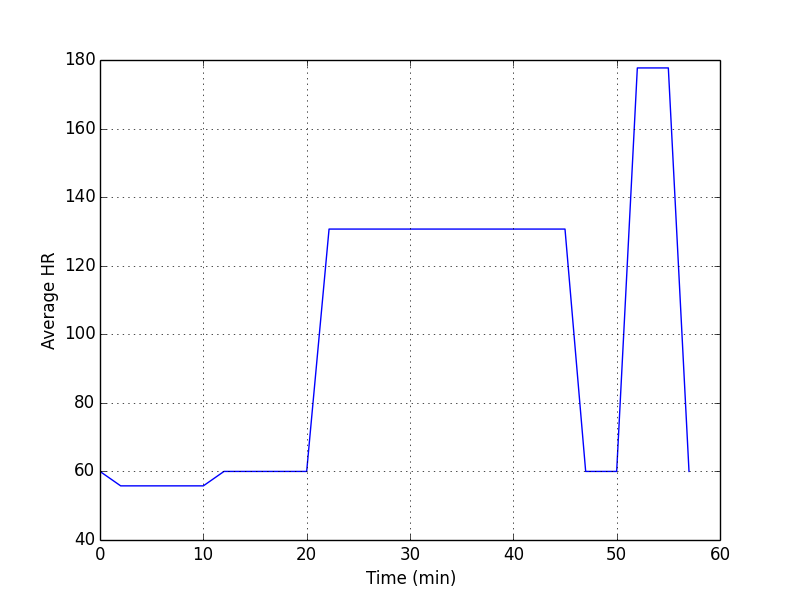
\includegraphics[height=3in,width=4in]{sim/hr} 
		\caption{HR Simulation Output.\label{fig:sim_hr}} 
	\end{center} 
\end{figure}

\begin{figure}[H]
	\centering
	\begin{subfigure}[b]{0.3\textwidth}
		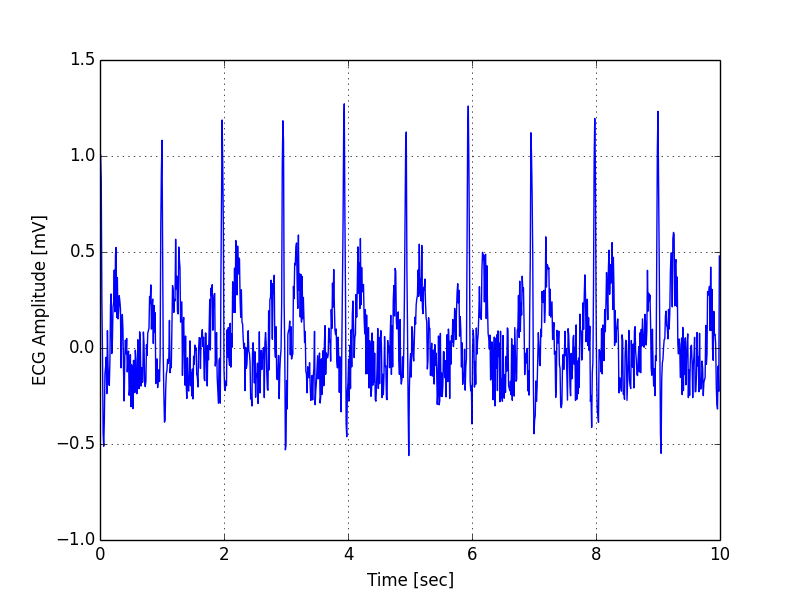
\includegraphics[width=\textwidth]{sim/ecg_1}
		%\caption{A gull}
		%\label{fig:gull}
	\end{subfigure}
	\begin{subfigure}[b]{0.3\textwidth}
		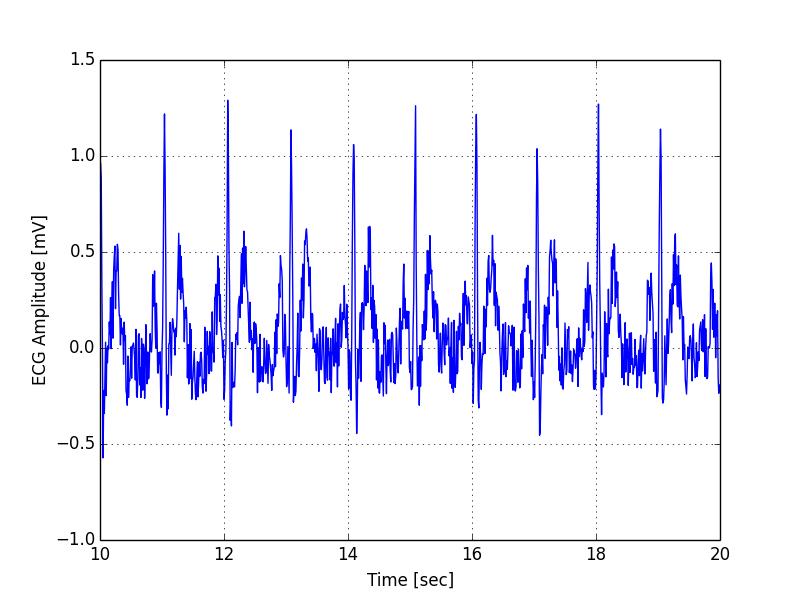
\includegraphics[width=\textwidth]{sim/ecg_2}
		%\caption{A tiger}
		%\label{fig:tiger}
	\end{subfigure}
	\begin{subfigure}[b]{0.3\textwidth}
		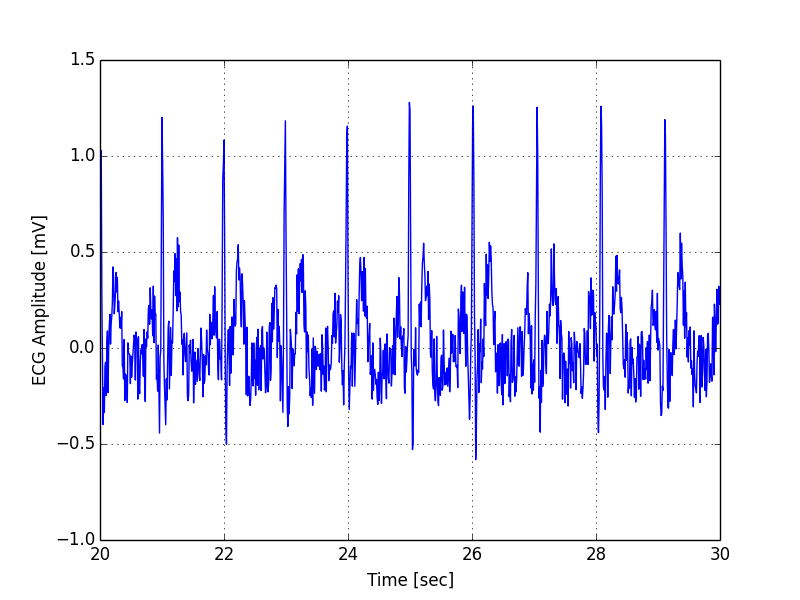
\includegraphics[width=\textwidth]{sim/ecg_3}
		%\caption{A mouse}
		%\label{fig:mouse}
	\end{subfigure}
	%\caption{Pictures of animals}\label{fig:animals}	
\end{figure}

\begin{figure}[H]
	\centering
	\begin{subfigure}[b]{0.3\textwidth}
		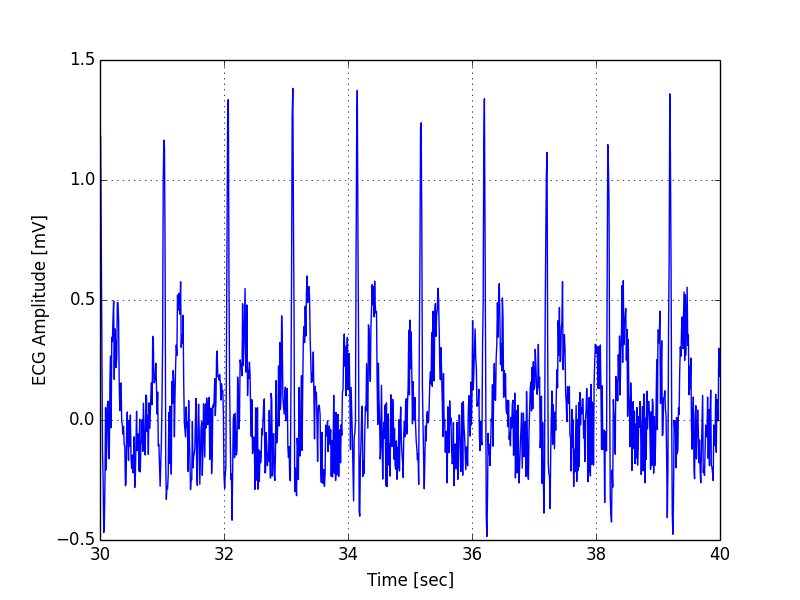
\includegraphics[width=\textwidth]{sim/ecg_4}
	\end{subfigure}
	\begin{subfigure}[b]{0.3\textwidth}
		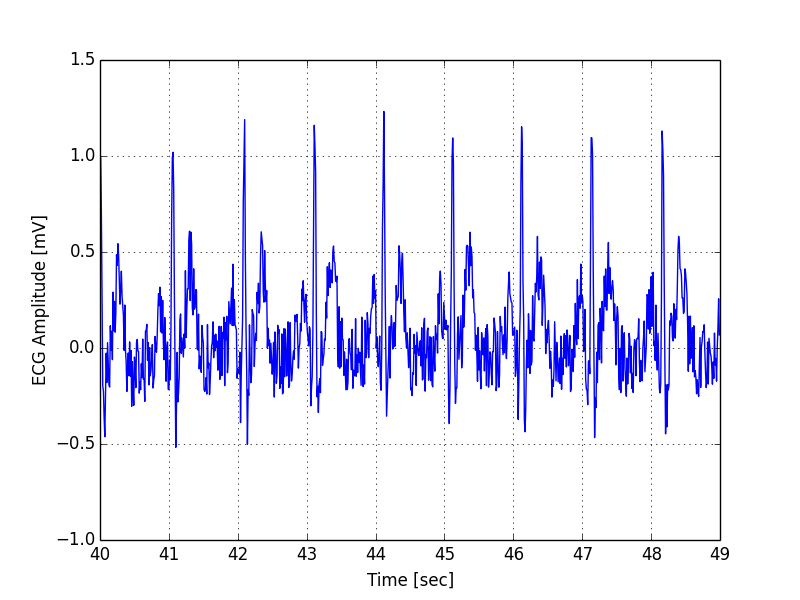
\includegraphics[width=\textwidth]{sim/ecg_5}
	\end{subfigure}
	\begin{subfigure}[b]{0.3\textwidth}
		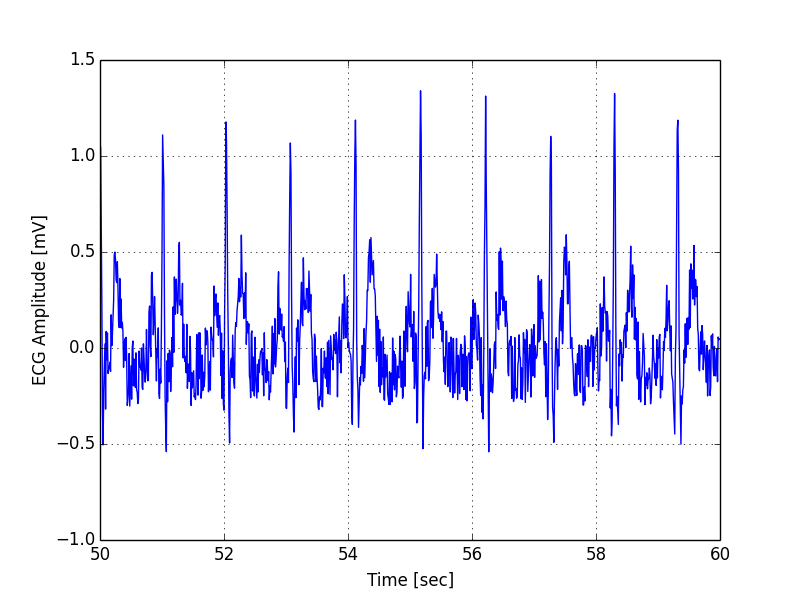
\includegraphics[width=\textwidth]{sim/ecg_6}
	\end{subfigure}
	%\caption{Pictures of animals}\label{fig:animals}	
\end{figure}

\begin{figure}[H]
	\centering
	\begin{subfigure}[b]{0.3\textwidth}
		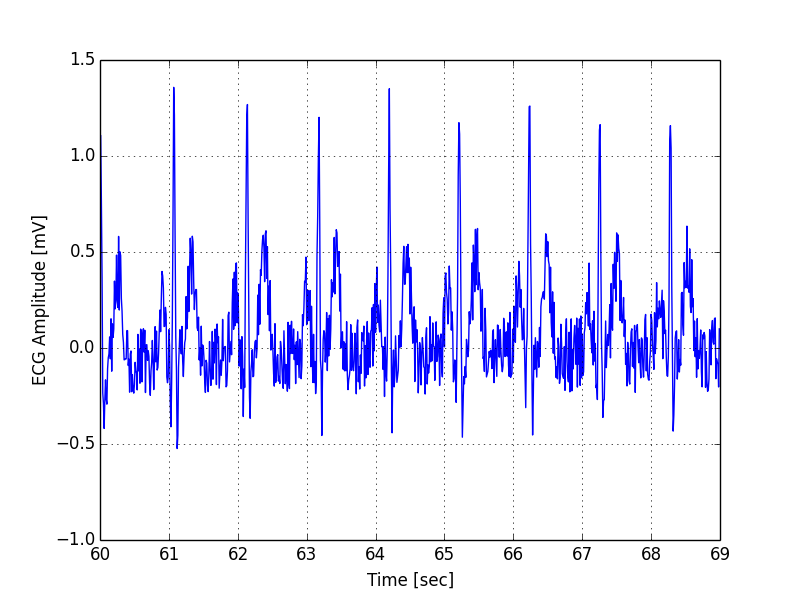
\includegraphics[width=\textwidth]{sim/ecg_7}
	\end{subfigure}
	\begin{subfigure}[b]{0.3\textwidth}
		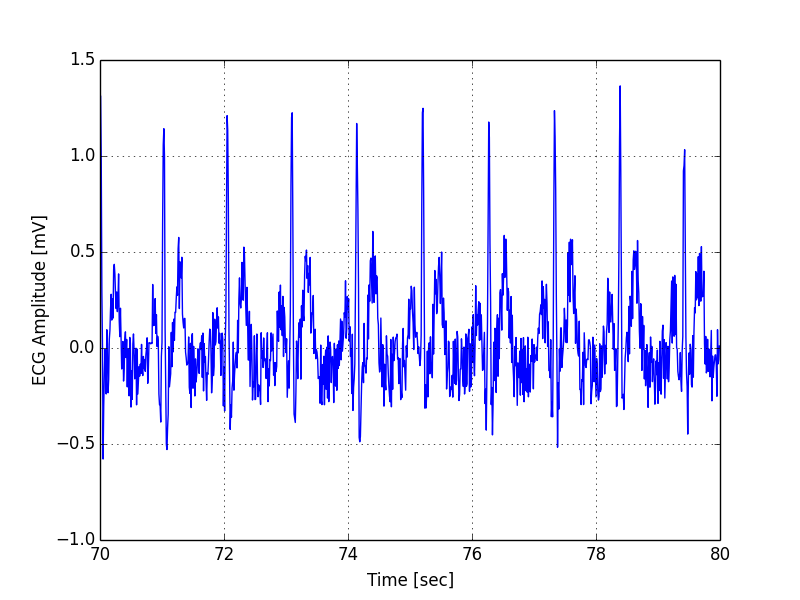
\includegraphics[width=\textwidth]{sim/ecg_8}
	\end{subfigure}
	\begin{subfigure}[b]{0.3\textwidth}
		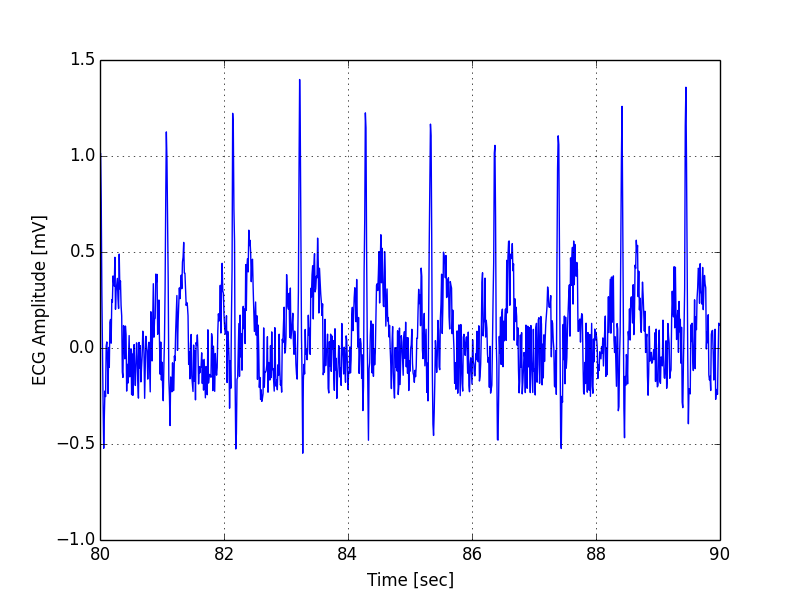
\includegraphics[width=\textwidth]{sim/ecg_9}
	\end{subfigure}
	%\caption{Pictures of animals}\label{fig:animals}	
\end{figure}

\begin{figure}[H]
	\centering
	\begin{subfigure}[b]{0.3\textwidth}
		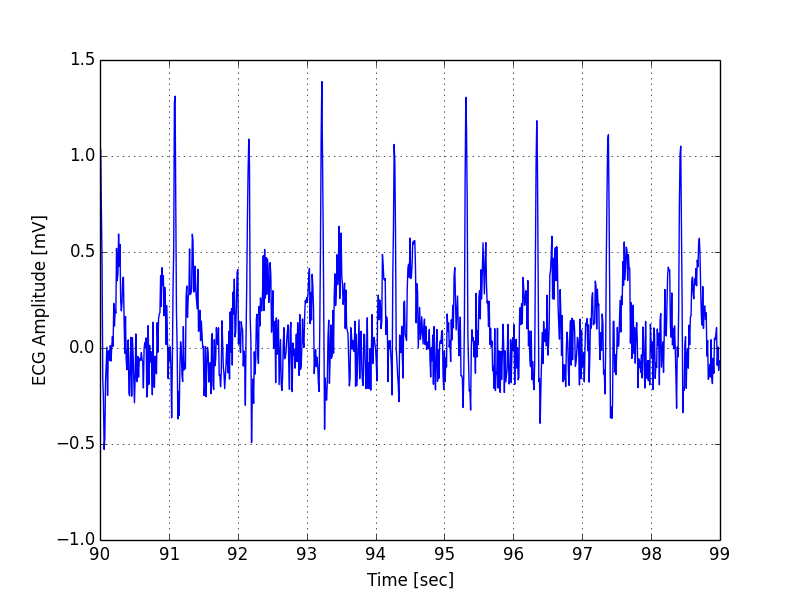
\includegraphics[width=\textwidth]{sim/ecg_10}
	\end{subfigure}
	\begin{subfigure}[b]{0.3\textwidth}
		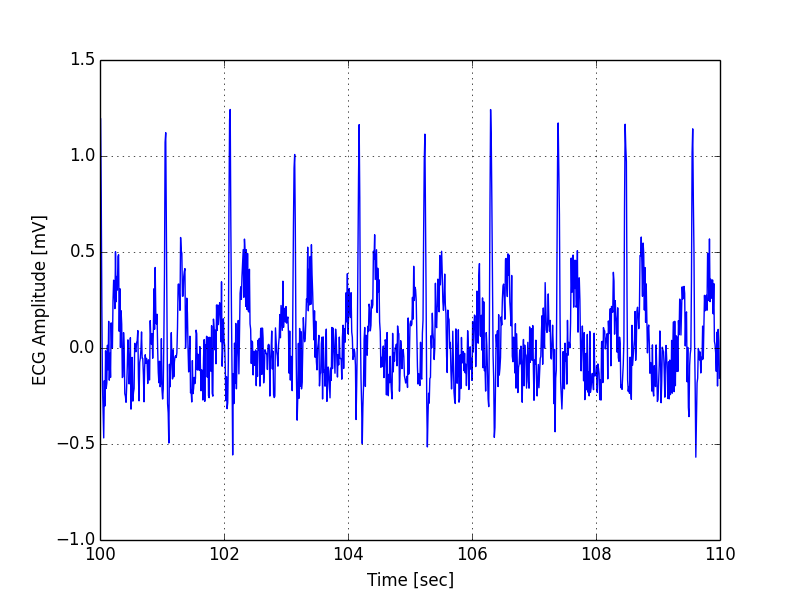
\includegraphics[width=\textwidth]{sim/ecg_11}
	\end{subfigure}
	\begin{subfigure}[b]{0.3\textwidth}
		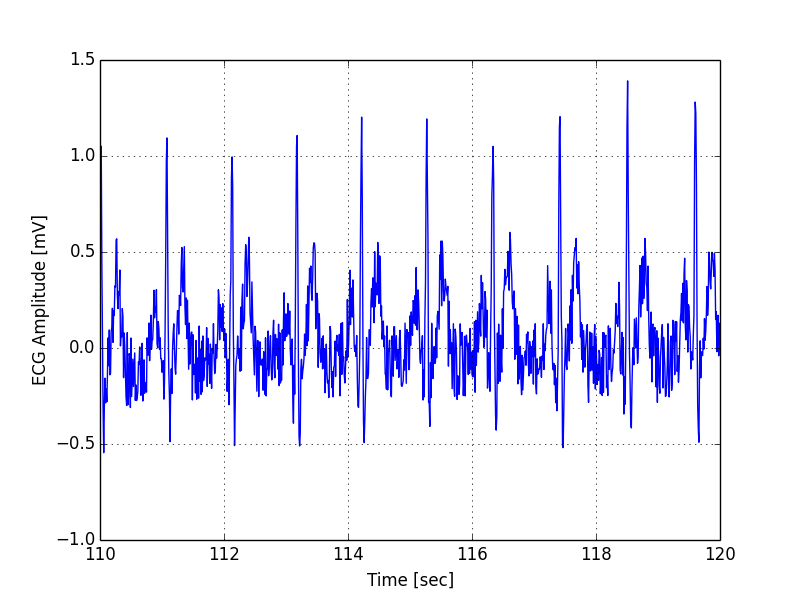
\includegraphics[width=\textwidth]{sim/ecg_12}
	\end{subfigure}
	%\caption{Pictures of animals}\label{fig:animals}	
\end{figure}

\begin{figure}[H]
	\centering
	\begin{subfigure}[b]{0.3\textwidth}
		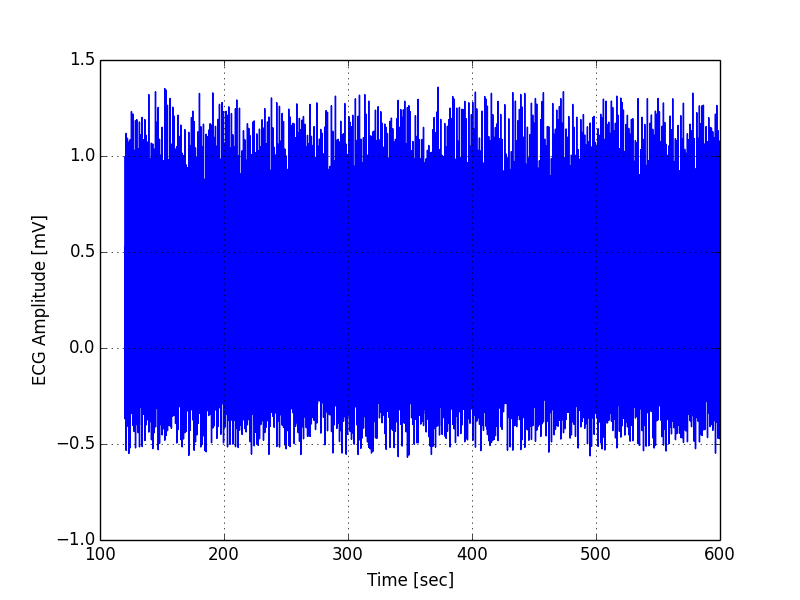
\includegraphics[width=\textwidth]{sim/ecg_13}
	\end{subfigure}
	\begin{subfigure}[b]{0.3\textwidth}
		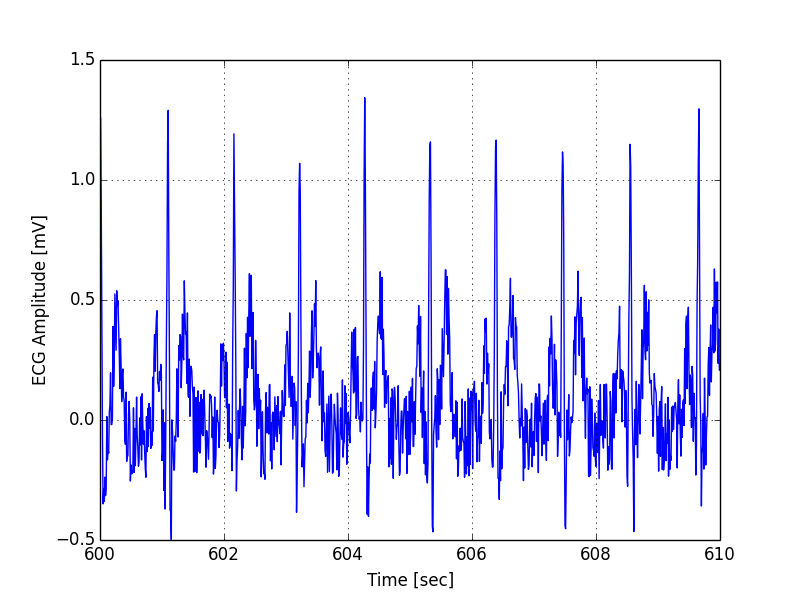
\includegraphics[width=\textwidth]{sim/ecg_14}
	\end{subfigure}
	\begin{subfigure}[b]{0.3\textwidth}
		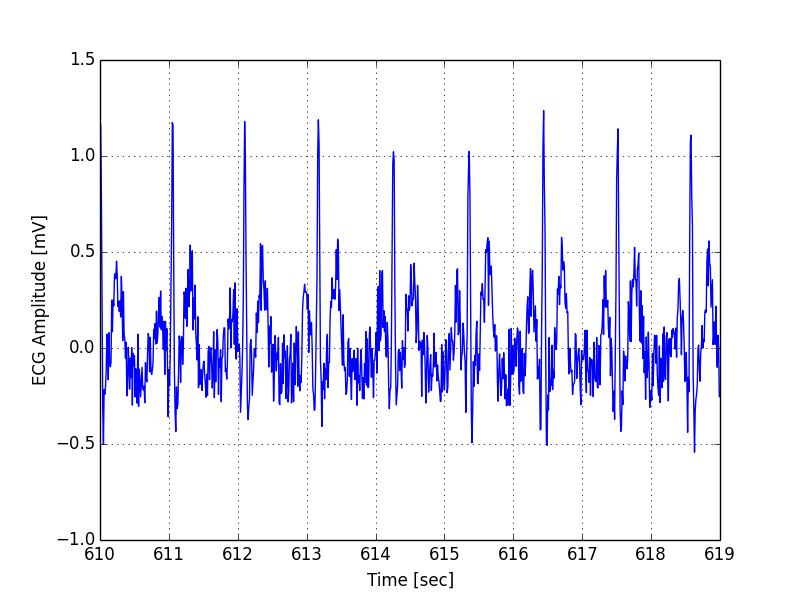
\includegraphics[width=\textwidth]{sim/ecg_15}
	\end{subfigure}
	%\caption{Pictures of animals}\label{fig:animals}	
\end{figure}

\begin{figure}[H]
	\centering
	\begin{subfigure}[b]{0.3\textwidth}
		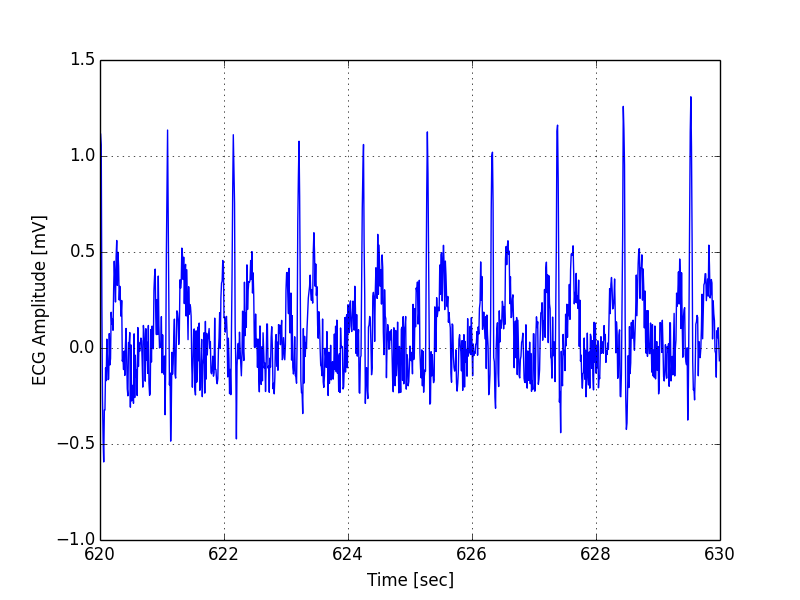
\includegraphics[width=\textwidth]{sim/ecg_16}
	\end{subfigure}
	\begin{subfigure}[b]{0.3\textwidth}
		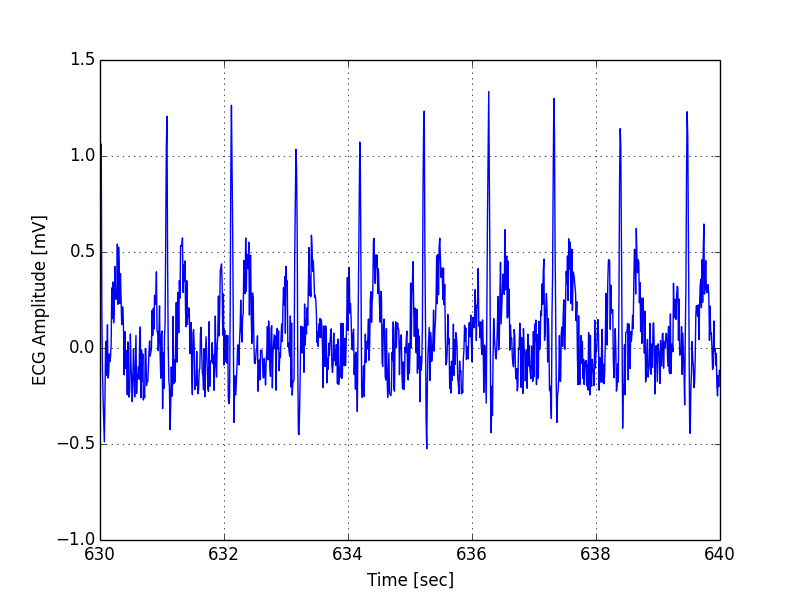
\includegraphics[width=\textwidth]{sim/ecg_17}
	\end{subfigure}
	\begin{subfigure}[b]{0.3\textwidth}
		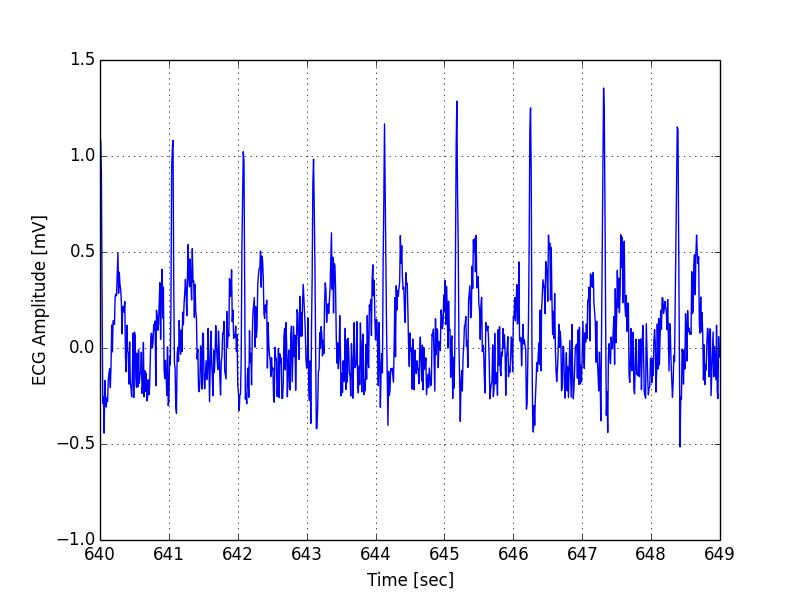
\includegraphics[width=\textwidth]{sim/ecg_18}
	\end{subfigure}
	%\caption{Pictures of animals}\label{fig:animals}	
\end{figure}

\begin{figure}[H]
	\centering
	\begin{subfigure}[b]{0.3\textwidth}
		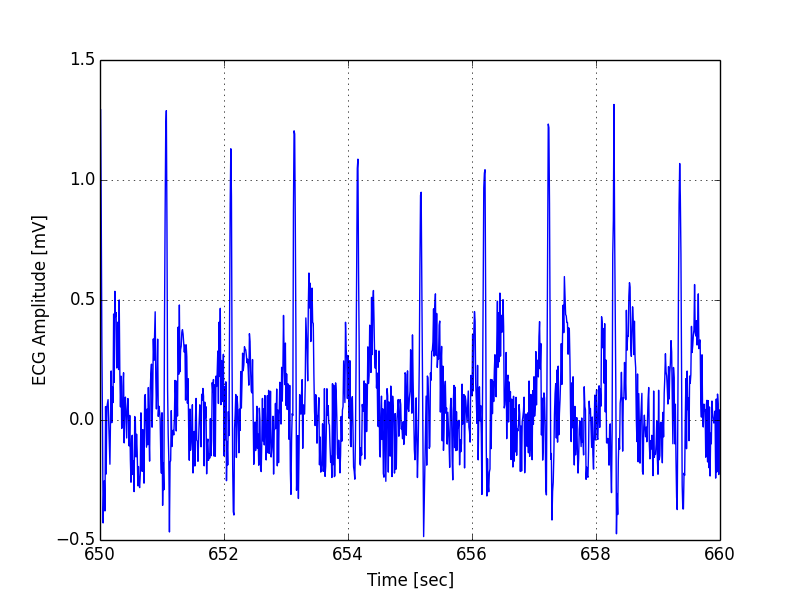
\includegraphics[width=\textwidth]{sim/ecg_19}
	\end{subfigure}
	\begin{subfigure}[b]{0.3\textwidth}
		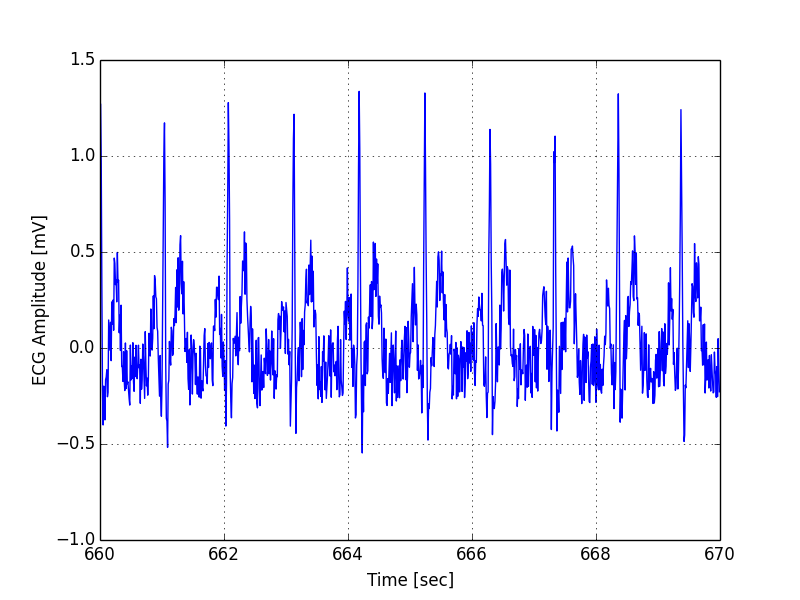
\includegraphics[width=\textwidth]{sim/ecg_20}
	\end{subfigure}
	\begin{subfigure}[b]{0.3\textwidth}
		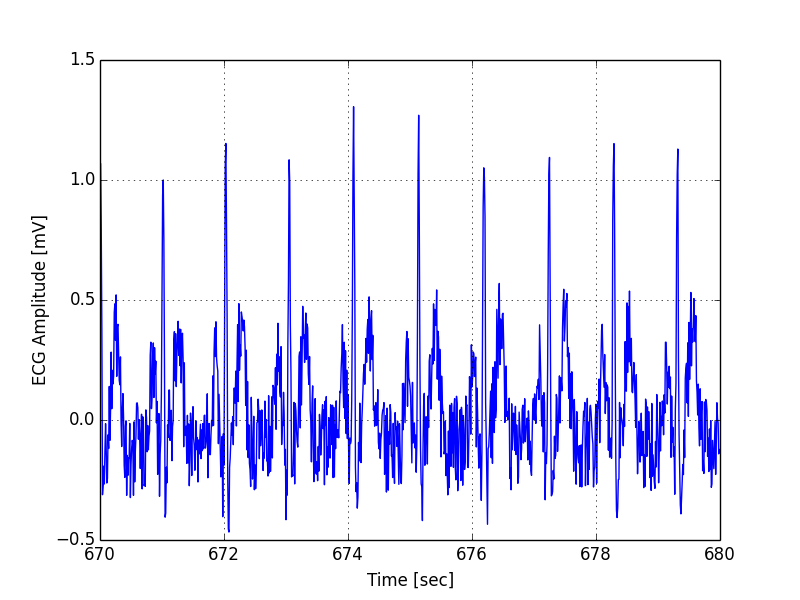
\includegraphics[width=\textwidth]{sim/ecg_21}
	\end{subfigure}
	%\caption{Pictures of animals}\label{fig:animals}	
\end{figure}

\begin{figure}[H]
	\centering
	\begin{subfigure}[b]{0.3\textwidth}
		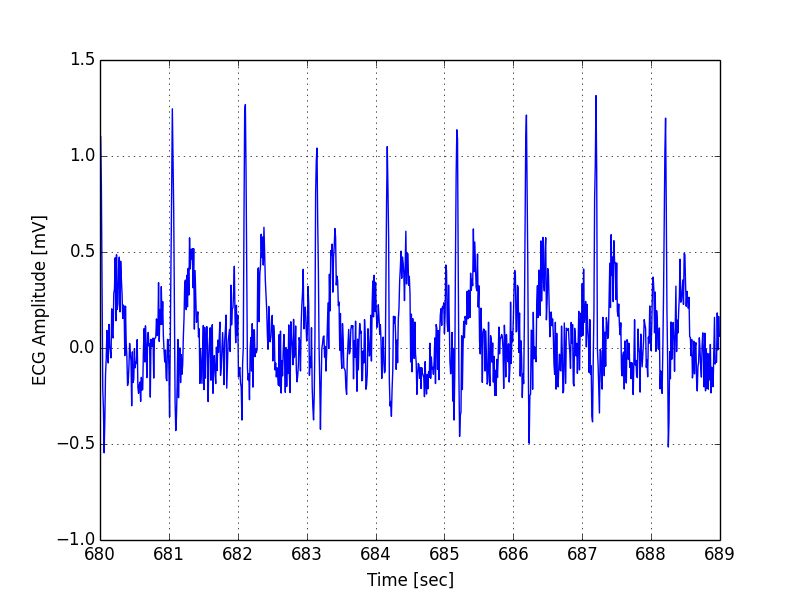
\includegraphics[width=\textwidth]{sim/ecg_22}
	\end{subfigure}
	\begin{subfigure}[b]{0.3\textwidth}
		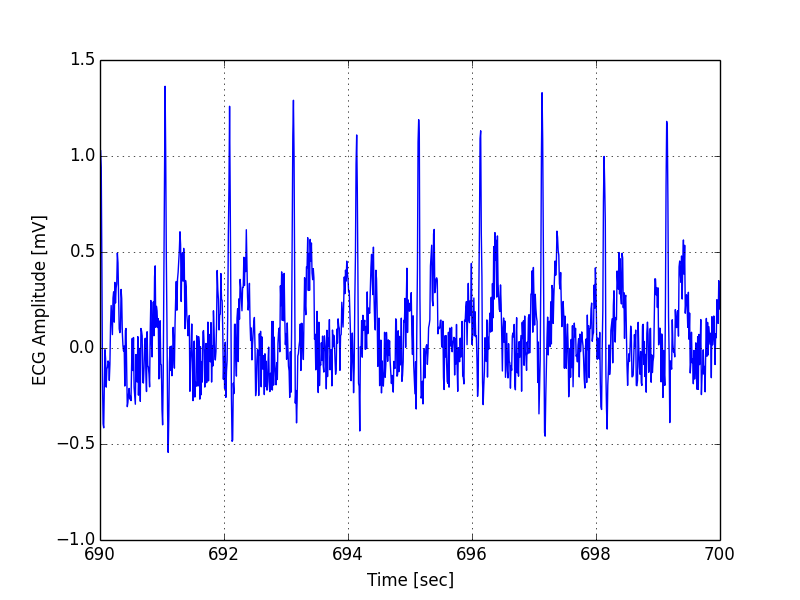
\includegraphics[width=\textwidth]{sim/ecg_23}
	\end{subfigure}
	\begin{subfigure}[b]{0.3\textwidth}
		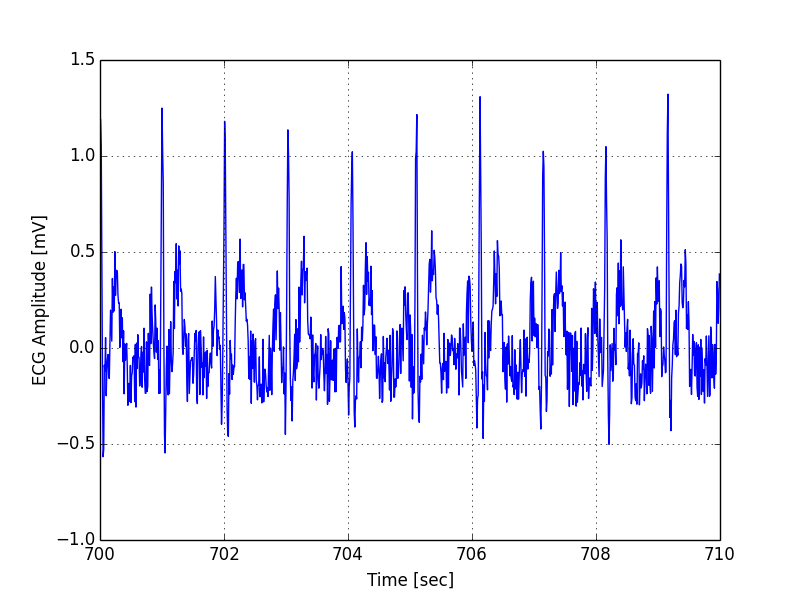
\includegraphics[width=\textwidth]{sim/ecg_24}
	\end{subfigure}
	%\caption{Pictures of animals}\label{fig:animals}	
\end{figure}

\begin{figure}[H]
	\centering
	\begin{subfigure}[b]{0.3\textwidth}
		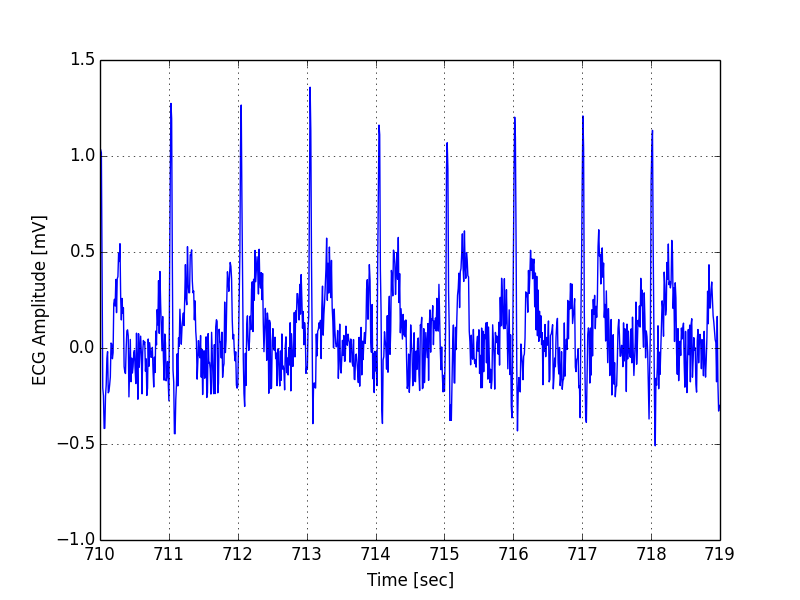
\includegraphics[width=\textwidth]{sim/ecg_25}
	\end{subfigure}
	\begin{subfigure}[b]{0.3\textwidth}
		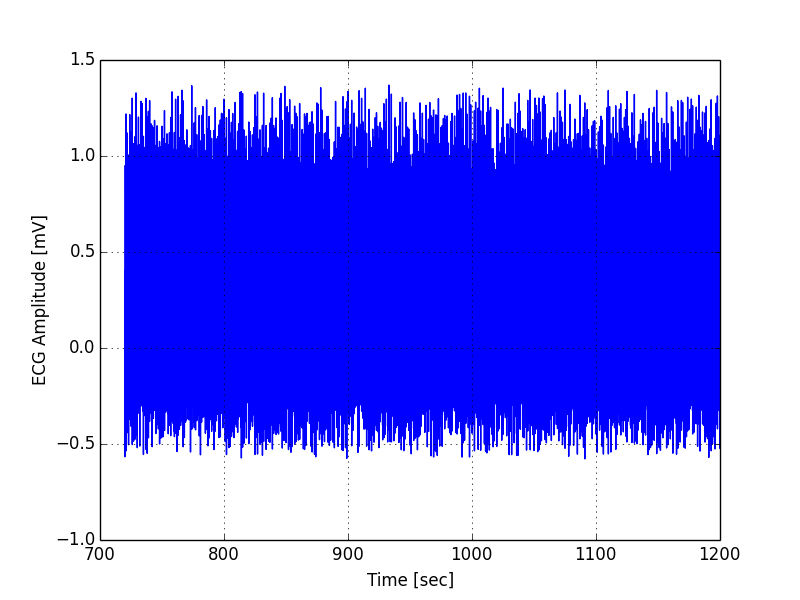
\includegraphics[width=\textwidth]{sim/ecg_26}
	\end{subfigure}
	\begin{subfigure}[b]{0.3\textwidth}
		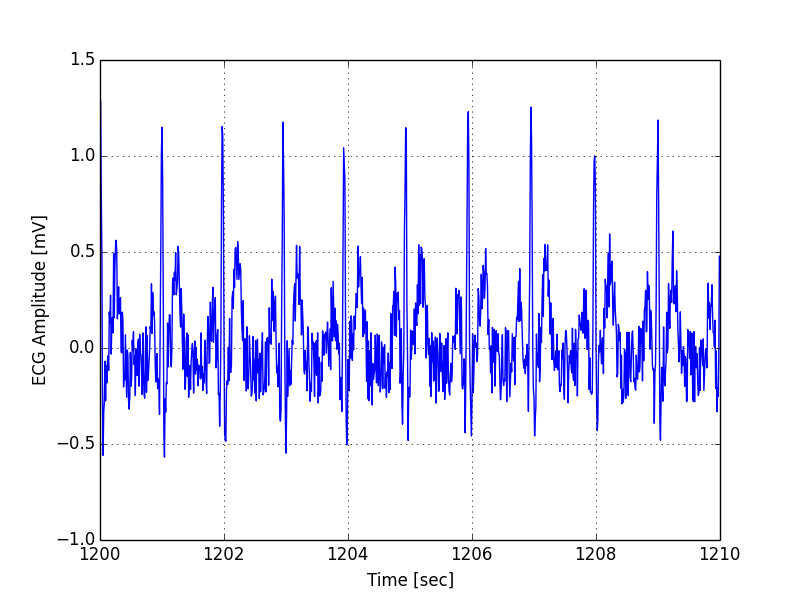
\includegraphics[width=\textwidth]{sim/ecg_27}
	\end{subfigure}
	%\caption{Pictures of animals}\label{fig:animals}	
\end{figure}

\begin{figure}[H]
	\centering
	\begin{subfigure}[b]{0.3\textwidth}
		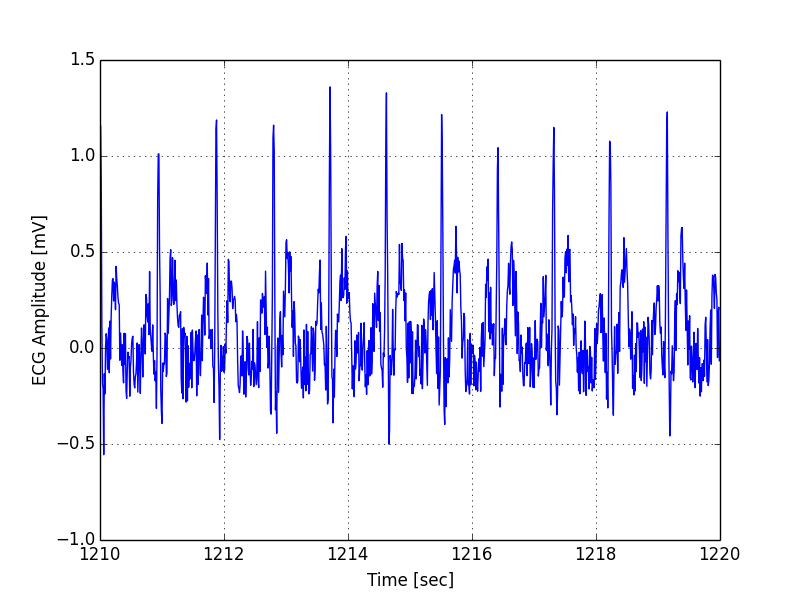
\includegraphics[width=\textwidth]{sim/ecg_28}
	\end{subfigure}
	\begin{subfigure}[b]{0.3\textwidth}
		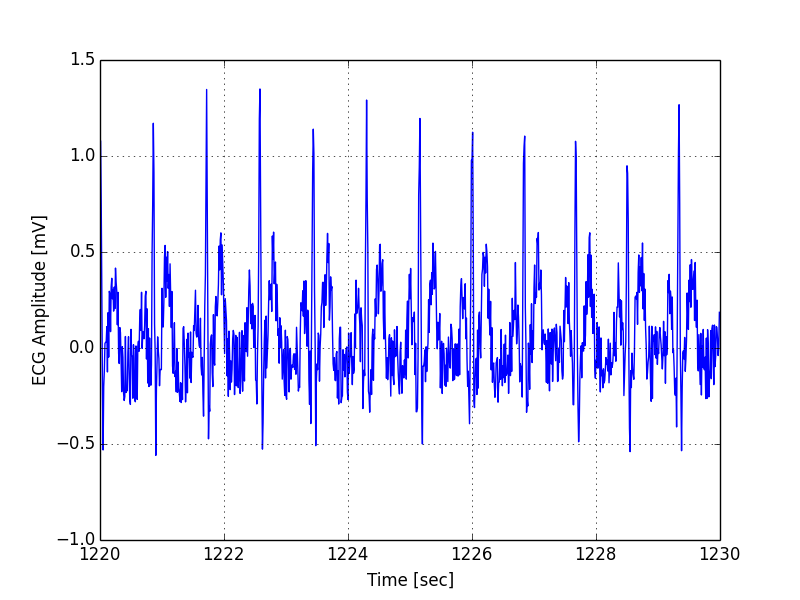
\includegraphics[width=\textwidth]{sim/ecg_29}
	\end{subfigure}
	\begin{subfigure}[b]{0.3\textwidth}
		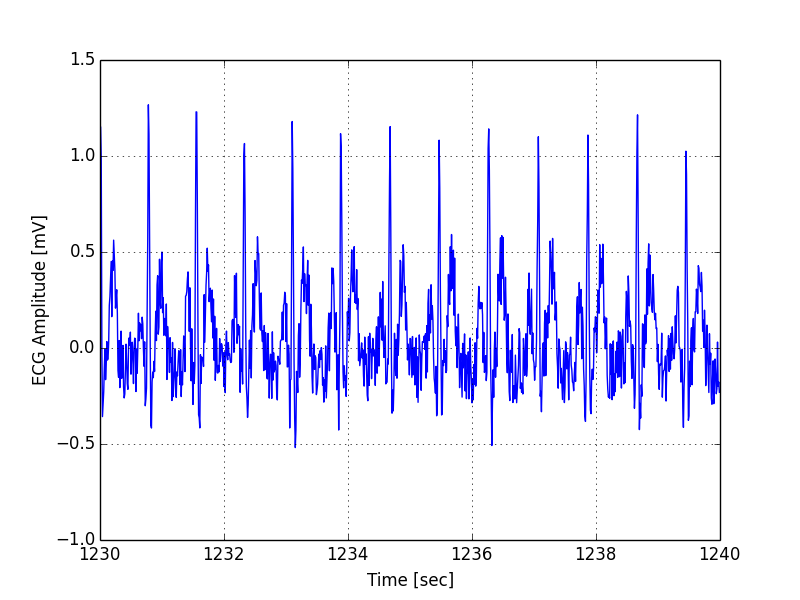
\includegraphics[width=\textwidth]{sim/ecg_30}
	\end{subfigure}
	%\caption{Pictures of animals}\label{fig:animals}	
\end{figure}

\begin{figure}[H]
	\centering
	\begin{subfigure}[b]{0.3\textwidth}
		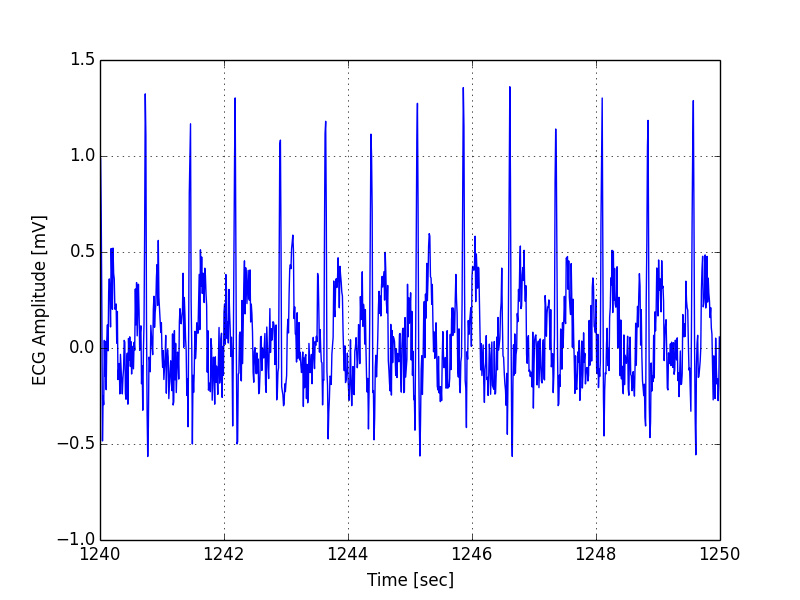
\includegraphics[width=\textwidth]{sim/ecg_31}
	\end{subfigure}
	\begin{subfigure}[b]{0.3\textwidth}
		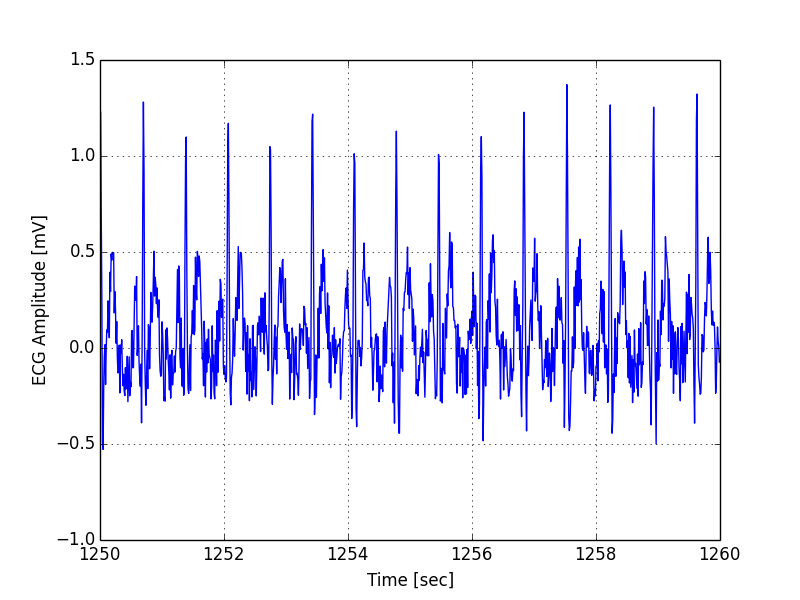
\includegraphics[width=\textwidth]{sim/ecg_32}
	\end{subfigure}
	\begin{subfigure}[b]{0.3\textwidth}
		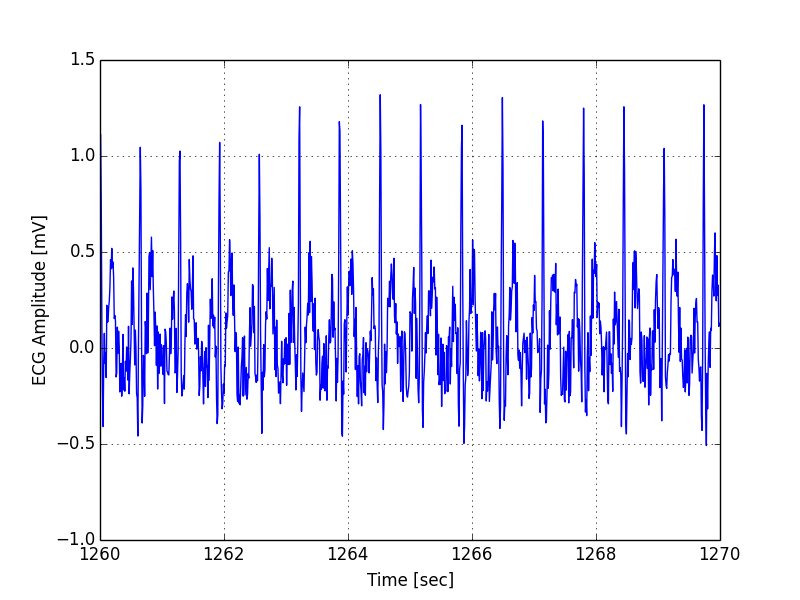
\includegraphics[width=\textwidth]{sim/ecg_33}
	\end{subfigure}
	%\caption{Pictures of animals}\label{fig:animals}	
\end{figure}

\begin{figure}[H]
	\centering
	\begin{subfigure}[b]{0.3\textwidth}
		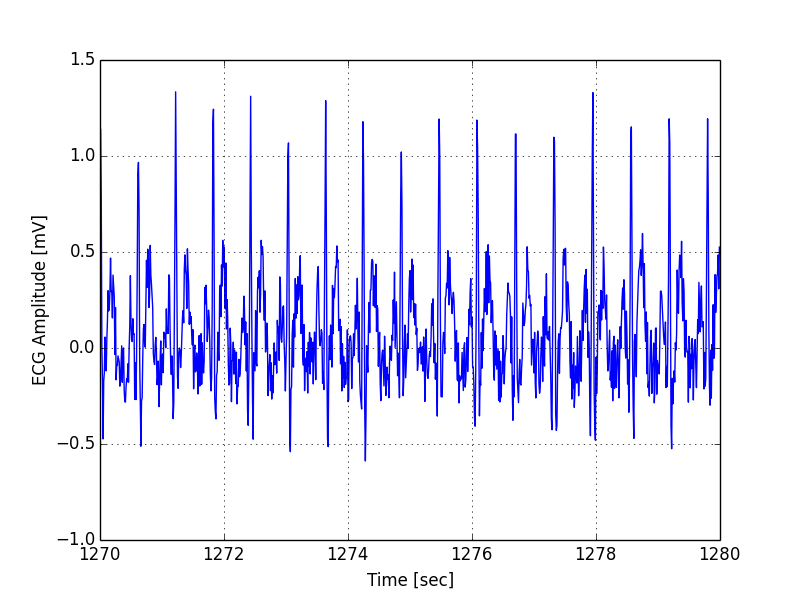
\includegraphics[width=\textwidth]{sim/ecg_34}
	\end{subfigure}
	\begin{subfigure}[b]{0.3\textwidth}
		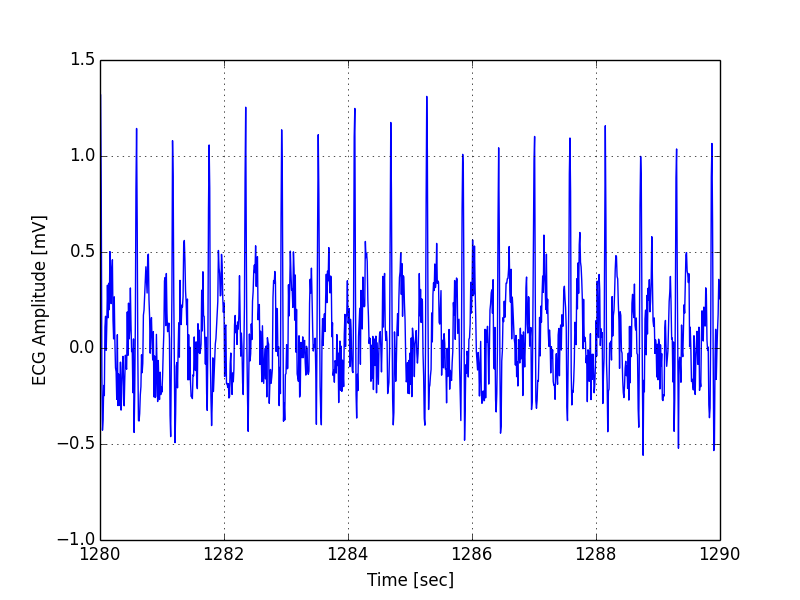
\includegraphics[width=\textwidth]{sim/ecg_35}
	\end{subfigure}
	\begin{subfigure}[b]{0.3\textwidth}
		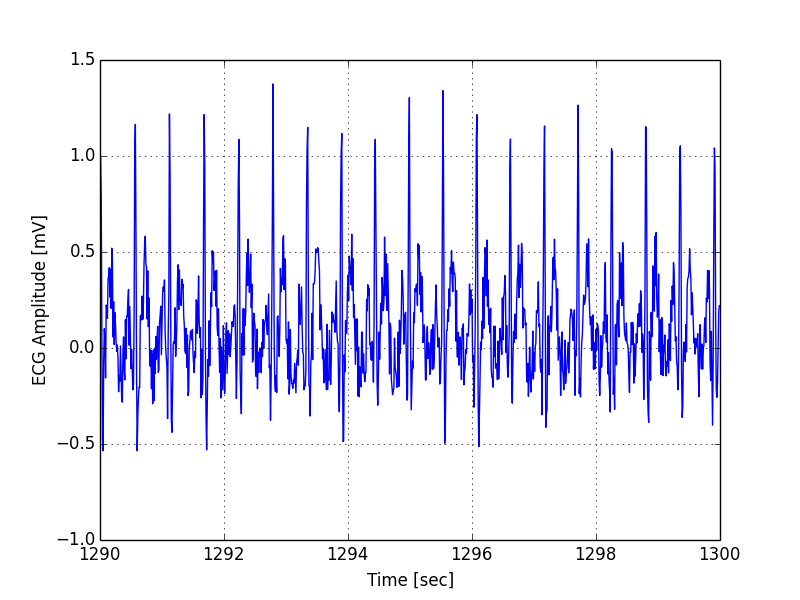
\includegraphics[width=\textwidth]{sim/ecg_36}
	\end{subfigure}
	%\caption{Pictures of animals}\label{fig:animals}	
\end{figure}

\begin{figure}[H]
	\centering
	\begin{subfigure}[b]{0.3\textwidth}
		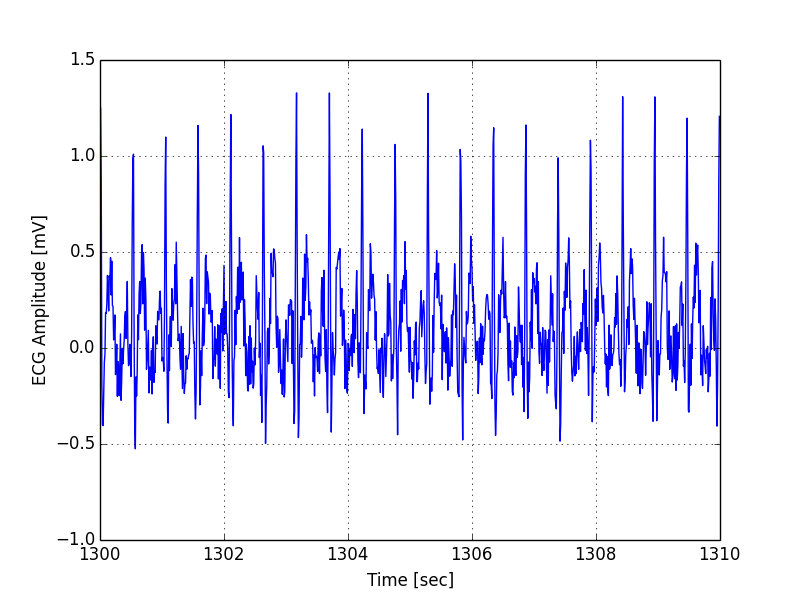
\includegraphics[width=\textwidth]{sim/ecg_37}
	\end{subfigure}
	\begin{subfigure}[b]{0.3\textwidth}
		\includegraphics[width=\textwidth]{sim/ecg_38}
	\end{subfigure}
	\begin{subfigure}[b]{0.3\textwidth}
		\includegraphics[width=\textwidth]{sim/ecg_39}
	\end{subfigure}
	%\caption{Pictures of animals}\label{fig:animals}	
\end{figure}

\begin{figure}[H]
	\centering
	\begin{subfigure}[b]{0.3\textwidth}
		\includegraphics[width=\textwidth]{sim/ecg_40}
	\end{subfigure}
	\begin{subfigure}[b]{0.3\textwidth}
		\includegraphics[width=\textwidth]{sim/ecg_41}
	\end{subfigure}
	\begin{subfigure}[b]{0.3\textwidth}
		\includegraphics[width=\textwidth]{sim/ecg_42}
	\end{subfigure}
	%\caption{Pictures of animals}\label{fig:animals}	
\end{figure}

\begin{figure}[H]
	\centering
	\begin{subfigure}[b]{0.3\textwidth}
		\includegraphics[width=\textwidth]{sim/ecg_43}
	\end{subfigure}
	\begin{subfigure}[b]{0.3\textwidth}
		\includegraphics[width=\textwidth]{sim/ecg_44}
	\end{subfigure}
	\begin{subfigure}[b]{0.3\textwidth}
		\includegraphics[width=\textwidth]{sim/ecg_45}
	\end{subfigure}
	%\caption{Pictures of animals}\label{fig:animals}	
\end{figure}

\begin{figure}[H]
	\centering
	\begin{subfigure}[b]{0.3\textwidth}
		\includegraphics[width=\textwidth]{sim/ecg_46}
	\end{subfigure}
	\begin{subfigure}[b]{0.3\textwidth}
		\includegraphics[width=\textwidth]{sim/ecg_47}
	\end{subfigure}
	\begin{subfigure}[b]{0.3\textwidth}
		\includegraphics[width=\textwidth]{sim/ecg_48}
	\end{subfigure}
	%\caption{Pictures of animals}\label{fig:animals}	
\end{figure}

\begin{figure}[H]
	\centering
	\begin{subfigure}[b]{0.3\textwidth}
		\includegraphics[width=\textwidth]{sim/ecg_49}
	\end{subfigure}
	\begin{subfigure}[b]{0.3\textwidth}
		\includegraphics[width=\textwidth]{sim/ecg_50}
	\end{subfigure}
	\begin{subfigure}[b]{0.3\textwidth}
		\includegraphics[width=\textwidth]{sim/ecg_51}
	\end{subfigure}
	%\caption{Pictures of animals}\label{fig:animals}	
\end{figure}

\begin{figure}[H]
	\centering
	\begin{subfigure}[b]{0.3\textwidth}
		\includegraphics[width=\textwidth]{sim/ecg_52}
	\end{subfigure}
	\begin{subfigure}[b]{0.3\textwidth}
		\includegraphics[width=\textwidth]{sim/ecg_53}
	\end{subfigure}
	\begin{subfigure}[b]{0.3\textwidth}
		\includegraphics[width=\textwidth]{sim/ecg_54}
	\end{subfigure}
	%\caption{Pictures of animals}\label{fig:animals}	
\end{figure}

\begin{figure}[H]
	\centering
	\begin{subfigure}[b]{0.3\textwidth}
		\includegraphics[width=\textwidth]{sim/ecg_55}
	\end{subfigure}
	\begin{subfigure}[b]{0.3\textwidth}
		\includegraphics[width=\textwidth]{sim/ecg_56}
	\end{subfigure}
	\begin{subfigure}[b]{0.3\textwidth}
		\includegraphics[width=\textwidth]{sim/ecg_57}
	\end{subfigure}
	%\caption{Pictures of animals}\label{fig:animals}	
\end{figure}

\begin{figure}[H]
	\centering
	\begin{subfigure}[b]{0.3\textwidth}
		\includegraphics[width=\textwidth]{sim/ecg_58}
	\end{subfigure}
	\begin{subfigure}[b]{0.3\textwidth}
		\includegraphics[width=\textwidth]{sim/ecg_59}
	\end{subfigure}
	\begin{subfigure}[b]{0.3\textwidth}
		\includegraphics[width=\textwidth]{sim/ecg_60}
	\end{subfigure}
	%\caption{Pictures of animals}\label{fig:animals}	
\end{figure}

\begin{figure}[H]
	\centering
	\begin{subfigure}[b]{0.3\textwidth}
		\includegraphics[width=\textwidth]{sim/ecg_61}
	\end{subfigure}
	\begin{subfigure}[b]{0.3\textwidth}
		\includegraphics[width=\textwidth]{sim/ecg_62}
	\end{subfigure}
	\begin{subfigure}[b]{0.3\textwidth}
		\includegraphics[width=\textwidth]{sim/ecg_63}
	\end{subfigure}
	%\caption{Pictures of animals}\label{fig:animals}	
\end{figure}

\begin{figure}[H]
	\centering
	\begin{subfigure}[b]{0.3\textwidth}
		\includegraphics[width=\textwidth]{sim/ecg_64}
	\end{subfigure}
	\begin{subfigure}[b]{0.3\textwidth}
		\includegraphics[width=\textwidth]{sim/ecg_65}
	\end{subfigure}
	\begin{subfigure}[b]{0.3\textwidth}
		\includegraphics[width=\textwidth]{sim/ecg_66}
	\end{subfigure}
	%\caption{Pictures of animals}\label{fig:animals}	
\end{figure}

\begin{figure}[H]
	\centering
	\begin{subfigure}[b]{0.3\textwidth}
		\includegraphics[width=\textwidth]{sim/ecg_67}
	\end{subfigure}
	\begin{subfigure}[b]{0.3\textwidth}
		\includegraphics[width=\textwidth]{sim/ecg_68}
	\end{subfigure}
	\begin{subfigure}[b]{0.3\textwidth}
		\includegraphics[width=\textwidth]{sim/ecg_69}
	\end{subfigure}
	%\caption{Pictures of animals}\label{fig:animals}	
\end{figure}

\begin{figure}[H]
	\centering
	\begin{subfigure}[b]{0.3\textwidth}
		\includegraphics[width=\textwidth]{sim/ecg_70}
	\end{subfigure}
	\begin{subfigure}[b]{0.3\textwidth}
		\includegraphics[width=\textwidth]{sim/ecg_71}
	\end{subfigure}
	\begin{subfigure}[b]{0.3\textwidth}
		\includegraphics[width=\textwidth]{sim/ecg_72}
	\end{subfigure}
	%\caption{Pictures of animals}\label{fig:animals}	
\end{figure}

\begin{figure}[H]
	\centering
	\begin{subfigure}[b]{0.3\textwidth}
		\includegraphics[width=\textwidth]{sim/ecg_73}
	\end{subfigure}
	\begin{subfigure}[b]{0.3\textwidth}
		\includegraphics[width=\textwidth]{sim/ecg_74}
	\end{subfigure}
	\begin{subfigure}[b]{0.3\textwidth}
		\includegraphics[width=\textwidth]{sim/ecg_75}
	\end{subfigure}
	%\caption{Pictures of animals}\label{fig:animals}	
\end{figure}

\begin{figure}[H]
	\centering
	\begin{subfigure}[b]{0.3\textwidth}
		\includegraphics[width=\textwidth]{sim/ecg_76}
	\end{subfigure}
	\begin{subfigure}[b]{0.3\textwidth}
		\includegraphics[width=\textwidth]{sim/ecg_77}
	\end{subfigure}
	%\caption{Pictures of animals}\label{fig:animals}	
\end{figure}

\end{appendices}  

%%%%%%%%%%%%%%%%%%%%%%%%%%%%%%%%%%%%%%%%%%%%%%%%%%%%%%%%%%%%%%%%%%%%%%%%%%%%%%%%%%%%%%%%%%%%%%%%%%%%
%%% Bibliography
\newpage
\bibliography{cse6730_project2_crocker_hasan_report} 
\bibliographystyle{ieeetr}
	
%%%%%%%%%%%%%%%%%%%%%%%%%%%%%%%%%%%%%%%%%%%%%%%%%%%%%%%%%%%%%%%%%%%%%%%%%%%%%%%%%%%%%%%%%%%%%%%%%%%%
%%% End document
\end{document}
